\documentclass[12pt]{svmono}
\usepackage{geometry}        
\geometry{letterpaper}    
\usepackage[parfill]{parskip}  
\usepackage{graphicx}
\usepackage{amssymb}
\usepackage{epstopdf}
\usepackage{appendix}
\DeclareGraphicsRule{.tif}{png}{.png}{`convert #1 `dirname #1`/`basename #1 .tif`.png}

\usepackage[colorlinks=true, pdfstartview=FitV, linkcolor=blue, 
            citecolor=blue, urlcolor=blue]{hyperref}

%\includeonly{Chapter1}
\usepackage{geometry}                		% See geometry.pdf to learn the layout options. There are lots.
\geometry{letterpaper}    
\usepackage{graphicx}
  \usepackage{amsmath}
  \usepackage{tikz}
 \usepackage{tcolorbox}
 \tcbuselibrary{skins}
 \tcbuselibrary{theorems}
\usepackage{hyperref}   
\usepackage{color}
\newcommand{\VAR}{CTRL-r }
%\usepackage[dvipsnames]{xcolor}
         		% ... or a4paper or a5paper or ... 
%\geometry{landscape}                		% Activate for for rotated page geometry
%\usepackage[parfill]{parskip}    		% Activate to begin paragraphs with an empty line rather than an indent
\usepackage{graphicx}				% Use pdf, png, jpg, or eps§ with pdflatex; use eps in DVI mode
								% TeX will automatically convert eps --> pdf in pdflatex		
\usepackage{amssymb}
\usepackage{epigraph}								% TeX will automatically convert eps --> pdf in pdflatex		
\usepackage{proof}

%\author{The Author}
%\date{}							% Activate to display a given date or no date
%\newcommand{\inp}[1]{\texttt{\colorbox{yellow!25}{#1}}}
\newcommand{\inp}[1]{\begin{tcolorbox}[colback=yellow!25!,colframe=black]\texttt{#1} \end{tcolorbox}}

%\newcommand{\proc}[1]{\texttt{\colorbox{green!25}{#1}}}
\newcommand{\proc}[1]{\begin{tcolorbox}[colback=green!35!white,colframe=black]#1 \end{tcolorbox}}
 \newcommand{\coq}[2]{\begin{tcolorbox}[bicolor,righthand width=\linewidth/4,colback=gray!10!white,colframe=black, ,colbacklower=orange ]$#1$ \tcblower
$ #2 \ $ \end{tcolorbox}}
 \newcommand{\coqtwo}[3]{
 \begin{tcolorbox}[bicolor,righthand width=\linewidth/4,sidebyside,colback=green!35!white,colbacklower=gray!10!white] {\small \texttt{#1}}\tcblower
]{\begin{tcolorbox}[bicolor,righthand width=\linewidth/4,colback=gray!10!white,colframe=black, ,colbacklower=orange ]$#2$ \tcblower
$ #3 \ $ \end{tcolorbox}}  \end{tcolorbox}}
 \newcommand{\rmk}[1]{
\begin{tcolorbox}[title= remark, colback=red!5!white,colframe=gray]
#1\end{tcolorbox}}
\newcommand{\mess}[1]{\begin{tcolorbox}[colback=white,colframe=black] #1 \end{tcolorbox}}
\newtheorem{Theorem}{Theorem}
\newtheorem{Lemma}{Lemma}
\newtheorem{Proposition}{Proposition}
\newtheorem{Definition}{Definition}
\newtheorem{Axiom}{Axiom}
\tcbuselibrary{breakable}


%\newtheorem{theorem}{Theorem}
%\newtheorem{corollary}[theorem]{Corollary}
%\newtheorem{definition}{Definition}
%\newtheorem{lemma}{Lemma}
%\newtheorem{exercise}{Exercise}
%\newtheorem{remark}{Remark}
%\newtheorem{example}{Example}
%\newtheorem{warning}{Warning}
\usepackage{subfiles}
\def\grad{ \mbox{grad}}
\def\curl{ \mbox{curl}}
\def\div{ \mbox{div}}
\def\U{\ensuremath {\cal U}}
\def\S{\ensuremath {\cal S}}
\def\V{\ensuremath {\cal V}}
\def\R{\ensuremath {\cal R}}
\def\tr{\ensuremath {\mbox{tr}}}




% ------------------- Title and Author -----------------------------
\title{Sample Book}
\author{Author}
\begin{document}


\frontmatter
\maketitle

\tableofcontents

 \frontmatter
\mainmatter
\chapter{Introduction}


\section{ Installation}

\subsection{Mac OSX}
\begin{enumerate}
\item Download and install  the latest version of Coq (it needs to be at least 8.6) from :

\href{https://coq.inria.fr/download}{https://coq.inria.fr/download}

Move it to your apps folder.


\item  Download and unpack spatchocq.app from canvas
move the spatchcoq.app to Applications and start it. 

\item when prompted find the Coq installation you have just move above. Navigate to 
\begin{verbatim}
/Applications/CoqIDE_8.6.app/Contents/Resources/bin/
\end{verbatim}
and choose coqtop. See Figure~\ref{fig:macos}

You only do this once.
\item  You only have to do this once. You might also need to install gtk, the simplest way to do this is  via homebrew
{\center brew install gtk+}
\begin{figure}\label{fig:macos}
\center
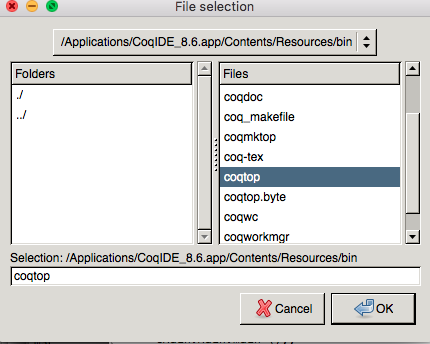
\includegraphics[scale=0.5]{Installation/macos.png}
\caption{Choose the Coq app in a Mac env}\label{fig:macos}
\end{figure}
\item enjoy

\end{enumerate}

\subsection{Windows}
\begin{enumerate}

\item get the zipfile spatchcoq.zip,  unzip it in a folder on a usb stick and doubleclick the application file spatchcoq. 
Note this version includes an instalation of Coq (not very extensively tested yet)

\item enjoy
\end{enumerate}


\subsection{Linux}
\begin{enumerate}
\item Download and install  the latest version of Coq it needs to be at least 8.6 so do not use 
apt-get install coq
\item  go to https://github.com/corneliuhoffman/spatchcoqocaml/tree/master
to build from scratch.
\item when prompted go to the Coq folder you just installed with opam and find  the application called {\bf coqtop}

\item enjoy
\end{enumerate}












%\section{Introducing the GUI}
\subsection{Online}

Figure~\ref{online gui}  is the main window in the online version.
Note however that, at this point, the online version is highly experimental.
\begin{enumerate}
\item The Green window  : This is the window that keeps the text that has already been processed.
\item The Yellow window ': This is the only window you can type your commands into.
\item The white window : this is the Coq feedback window. 
\item The grey window : this is a window for messages.
\item The run button: this sends the first line from the input window to Coq.
\item The undo button: this undoes the last command.
\end{enumerate}
\begin{figure}[h!]
\includegraphics[scale=0.3]{Installation/mainonline.png}
\caption{the online GUI}\label{online gui}
\end{figure}

\subsection{The menus}

The File menu (Figure \ref{file}) is quite standard:

\begin{figure}[h!]
\includegraphics[scale=0.5]{Installation/menu1online.png}


\caption{the File  Menu}\label{file}
\end{figure}

The action menu allows you to pick run, undo or print tree:

\begin{figure}[h!]
\includegraphics[scale=0.4]{Installation/menu3online.png}


\caption{the Action Menus}\label{actionsonline}
\end{figure}


The Tactics menu (Figure \ref{tacticsonline}) allows one to pick one of the predefined tactics. 
Note the place keeper VAR. 
These can be modified. More on these later.

\begin{figure}[h!]
\includegraphics[scale=0.5]{Installation/menu2online.png}


\caption{the Tactics Menus}\label{tacticsonline}
\end{figure}
\subsection{Keyboard shortcuts}

\begin{itemize}
\item CTRL-Space autocompletion
\item CTRL-r Run
\item CTRL-u Undo
\item CTRL-t Draw tree. 
\end{itemize}









\subsection{Desktop}
\subsubsection{Main windows}
Figure~\ref{first look} is a view of the GUI. As you can see there are 4 different windows and three buttons.
\begin{enumerate}
\item The Green window  : This is the window that keeps the text that has already been processed.
\item The Yellow window ': This is the only window you can type your commands into.
\item The Gray  window : this is the Coq feedback window. 
\item The White window : this is a window for messages.
\item The run button: this sends the first line from the input window to Coq.
\item The undo button: this undoes the last command.
\item The draw tree button: this draws the proof trees for all the completed theorems.
\item The symbol buttons: These allows one to type mathematical symbols.
\item The Search box/button: These allow searching for theorems by pattern.
\end{enumerate}


\begin{figure}[h!]
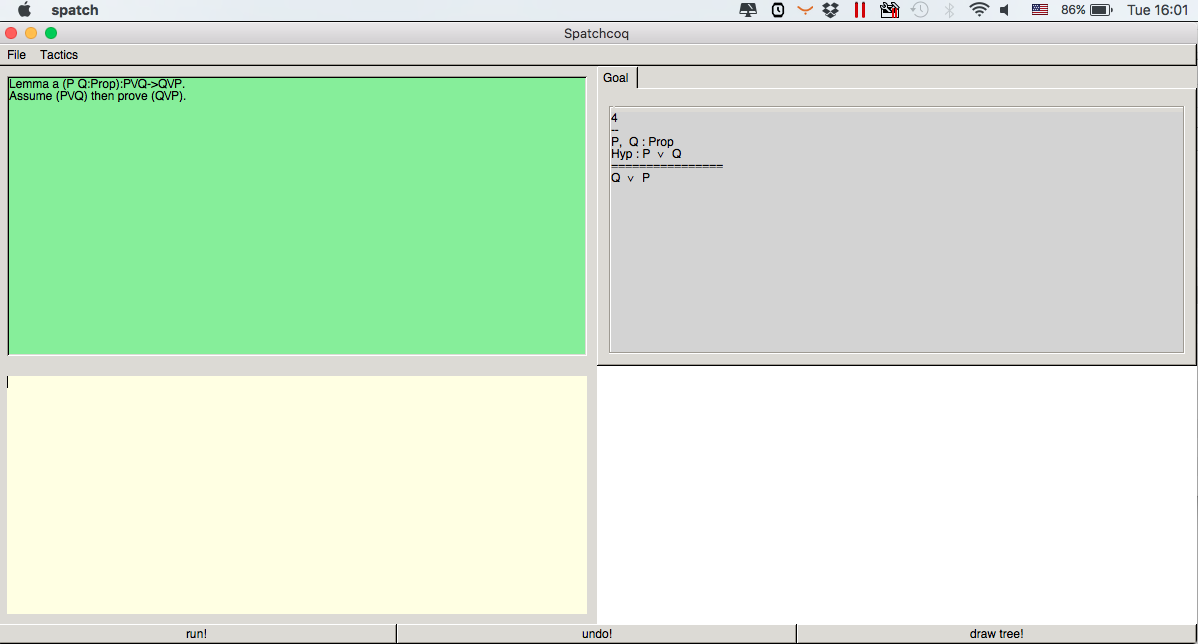
\includegraphics[scale=0.3]{Installation/main.png}
\caption{the GUI}\label{first look}
\end{figure}
\subsection{The menus}

The File menu (Figure \ref{file}) is quite standard:

\begin{figure}[h!]
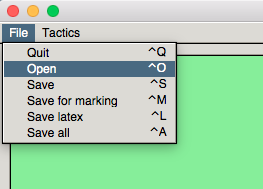
\includegraphics[scale=0.5]{Installation/menu1.png}


\caption{the File  Menu}\label{file}
\end{figure}

The Tactics menu (Figure \ref{tactics}) allows one to pick one of the predefined tactics. 
Note the place keeper VAR. 
These can be modified. More on these later.

\begin{figure}[h!]
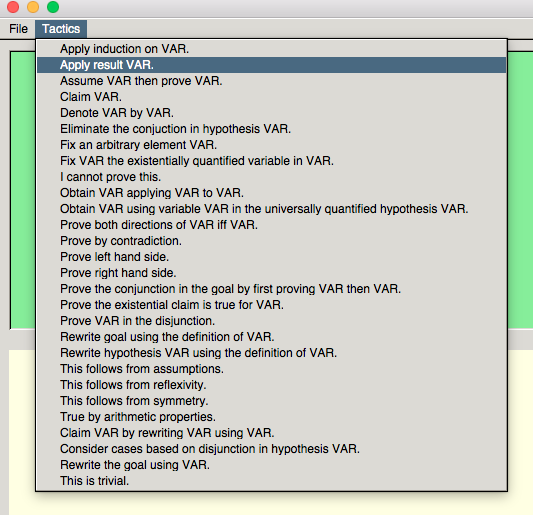
\includegraphics[scale=0.5]{Installation/menu2.png}


\caption{the Tactics/Environment Menus}\label{tactics}
\end{figure}
\subsection{Keyboard shortcuts}

Pressing ESC autocompletes the commands and pressing \VAR circles around the various possibilities for VAR.




%
\chapter{Two simple examples}\label{ch:examples}
We give two detailed examples that will exemplify the mechanics of the GUI. For clarity we will use colour boxes that will exemplify the window that we refer to. So green boxes refer to the processed window, yellow ones to the input window and gray ones to the feedback window.

\subsection{Propositional Calculus}

We will prove that if $P$ and $Q$ are propositions then $$P\lor Q \Rightarrow Q\lor P$$

the way to enter this is:

\inp{Lemma commor(P Q :Prop): P \texttt{\char`\\}/ Q -> Q \texttt{\char`\\}/ P .}
 
 Note that  the feedback from Coq says 
\coq{
P,  Q : Prop \\
}{
P  \lor  Q  \rightarrow  Q \lor  P 
}
This means that the hypotheses are that $P$ and $Q$ are propositions and the conclusion is $ P \lor Q \rightarrow Q \lor P$. To prove an implication  statement we assume the left hand and try to prove the right hand. Here is how you do it in Spatchcoq. There are two different ways to do this in spatchCoq:

Type ``Assume'' and press ESC to get a list of tactic choices:

\begin{figure}[h!]
\includegraphics[scale=0.5]{Installation/Escape.png}


\label{tactics}
\end{figure}

choose the tactic

\noindent
\inp{Assume VAR then prove VAR.}

Press \VAR to select the first VAR.

write $( P \lor Q )$ to replace the first VAR. Repeat \VAR and and replace the second VAR by $(Q \lor P)$.



The text in the yellow window should now be 

\noindent
\inp{Assume $( P \lor Q )$ then prove $( Q \lor P )$.}

Click run.


The other variant is to click on the orange goal in the feedback column to get a number of  to get a list of possible choices:
\begin{figure}[h!]
\includegraphics[scale=0.5]{Installation/clickgoal.png}
\label{tactics}
\end{figure}
Note that the choices bellow the horizontal line are tactics while those on the top are pieces of the goal. You can use a combination of the two methods of course. As before choose 
\inp{Assume $( P \lor Q )$ then prove $( Q \lor P )$.} and click run.


The response from Coq is

\coq{
 P \ Q: \mbox{Prop}\\
\mbox{Hyp}: P \lor Q
}{Q\lor P
}

This reflects the fact that we have a new hypothesis tabled Hyp  and a new conclusion.

Of course since we have a hypothesis with a disjunction we will use an argument by cases. To do so, type ``cases'' and press ESC. Choose the following:
\inp{Consider cases based on disjunction in hypothesis VAR.}

Press \VAR and replace VAR by Hyp. Click run.

Similarly click on the hypothesis Hyp on the right hand side to get:

\begin{figure}[h!]
\includegraphics[scale=0.5]{Installation/clickgoal1.png}
\label{tactics}
\end{figure}
 choose 
\inp{Consider cases based on disjunction in hypothesis Hyp .}

and click Run.

Notice that there are now two goals:
\coq{
 P \ Q: \mbox{Prop}\\
\mbox{Hyp0}: P\\
===========\\
}{
Q\lor P
}

and 

\coq{
P \ Q: \mbox{Prop}\\
\mbox{Hyp1}:  Q\\
===========
}{
Q\lor P
}

corresponding to the two cases to consider. In first goal we will prove the right hand side of the disjunction in the conclusion. To do so, type ``right'' and press ESC. You get to pick

\inp{
Prove right hand side.}

and after clicking run you will get the following feedback (note that the second goal stays unchanged)

\coq{
P \ Q: \mbox{Prop}\\
\mbox{Hyp0}: P\\
===========
}{
 P
}

Finally you can finish this goal by using the hypothesis Hyp0. To do this you use
\inp{This follows from assumptions.}

Note that you have now finished this goal. Repeat the argument for the second goal by using:

\inp{Prove left hand side.}
\inp{This follows from assumptions.}

to get \coq{ }{\text{no goals}}

Now type
\inp{Qed.}
to save the theorem. It now appears among the proved theorems:

and you can see its proof tree by clicking on draw tree:


\begin{figure}[h!]
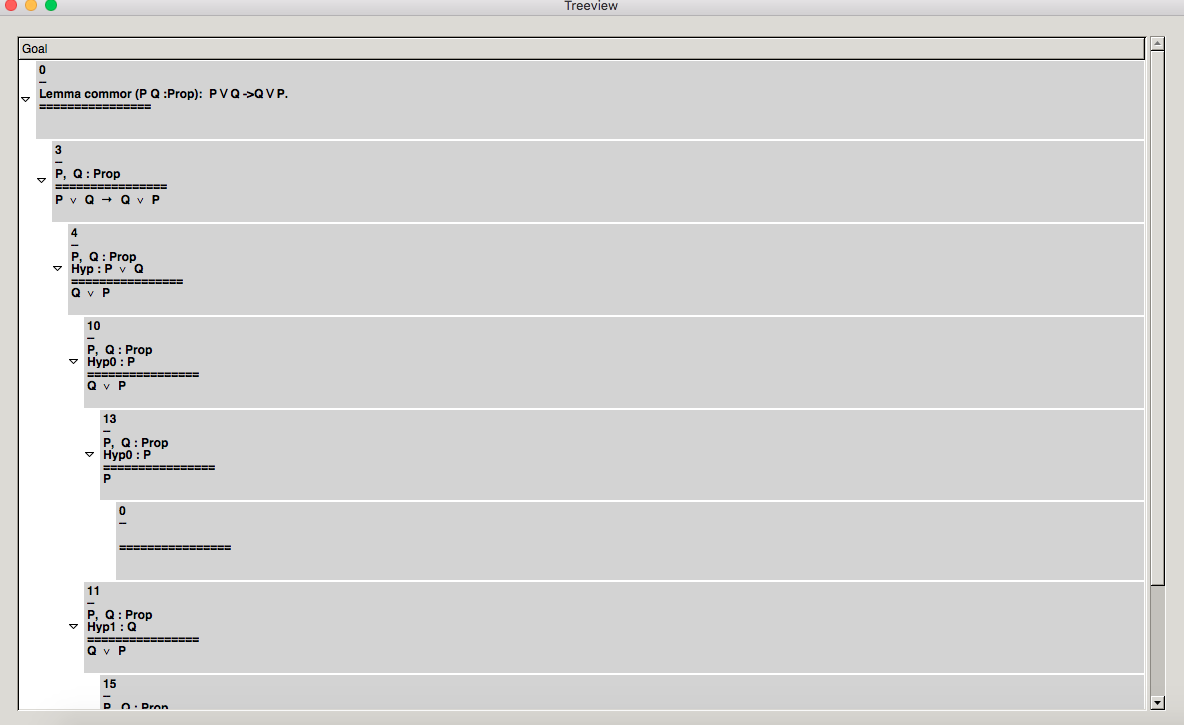
\includegraphics[scale=0.3]{Installation/treecommor.png}
\caption{the tree window}\label{treesearch}
\end{figure}

\subsection{An elementary number theory example}
We shall prove the transitivity of divisibility. That is we will prove that
$$\forall a,b, c \in \mathbb{N},  a |b \land b | c \Rightarrow a | c.$$

In the process we will introduce definitions and notations.

To start we note that we will be talking about objects of type \texttt{nat}. We weill introduce the following definition

\inp{Definition divides a b := exists x:nat, b = a*x.}

We hope that the format is quite clear, it resembles the one we used before but uses a few new notions, the operator \texttt{:=}
 which the defines the function \texttt{divides} and the quantifier \texttt{exists}. Note that we have not explicitly stated that a and b should be natural numbers, Coq will deduce that from the context. We could have been very precise as follows:
 \inp{ Definition divides (a b:nat) := exists x:nat, b = a*x.}

Note that the definition will not get any feedback from Coq. If we want to check that we have correctly defined our notion we can use
\inp{Check divides.}

to get

\mess{Query commands should not be inserted in
scripts\\

divides\\
     \texttt{: nat -> nat -> Prop}}
     
or
\inp{Print divides.}
to get a more detailed 
\mess{
Query commands should not be inserted in
scripts \\

divides = $\lambda a b : nat, \exists x : nat, b = a * x$\\
    \texttt{ : nat -> nat -> Prop}
\\
Argument scopes are [nat\_scope nat\_scope]
}
We will nod describe all this output here but we note the change from \texttt{exists} to $\exists$ and the occurrence of $\lambda$, a notation for functions.


Next we define a notation for divides

\inp{Notation " a | b " := (divides a b) (at level 10).}

Again no feedback from Coq. The definition should be self-evident except for the ``(at level 10)'' part. We will discuss this elsewhere.

We are now ready to state out theorem

We can state the theorem as (see the corresponding feedback)

\inp{Theorem refldiv (a b c:nat): \\ (a | b) $\land$ (b | c) -> (a |c).}

\coq{a,  b,  c : nat }{a  |  b  \land  b  |  c \rightarrow  a  |  c }

but we prefer the version

\inp{Theorem refldiv: forall a b c, (a | b) $\land$ (b | c) -> (a |c).
}
because it is  almost identical to the above mathematical statement and it will allow us to show some more tactics. The corresponding feedback is
\coq{ }{
\forall  a \  b\   c : nat,  a  |  b \  \land \ b  |  c\  \rightarrow\ a  |  c }

Note that Coq has correctly deduced that $a, b, c$ are natural numbers and replaced the quantifier \texttt{forall} with $\forall$. Note also that in this form there are no hypotheses.

We fill fix the three variables with the tactics:
\inp{Fix an arbitrary element a.\\
Fix an arbitrary element b.\\
Fix an arbitrary element c.}

to get 
\coq{a,  b,  c : nat \\
}{
a  |  b  \land  b  |  c \rightarrow  a  |  c }

As before, in order to prove an implication $A\rightarrow B$ we use the tactic

\inp{Assume A then prove B.}

More precisely, in this case we have
\inp{Assume (a | b $\land$ b | c ) then prove (a | c).}
to get

\coq {a,  b,  c : nat \\
Hyp : a  |  b  \land  b  |  c \\
}{
a  |  c }


Note that hypothesis Hyp is of type $A \land B$. We will split this in two hypotheses with:
\inp{Eliminate the conjuction in hypothesis Hyp.}
to get

\coq {a,  b,  c : nat \\
Hyp0 : a  |  b\\
Hyp1 :  b  |  c \\
}{
a  |  c }

We seem to have used all the tricks up our selves and so it is time to ``unfold'' the definitions:
\inp{Rewrite hypothesis Hyp0 using the definition of divides.}
\coq{a,  b,  c : nat \\
Hyp0 : \exists  x  :  nat,  b  =  a  *  x \\
Hyp1 :  b  |  c \\
}{
a  |  c }

then 
\inp{Rewrite hypothesis Hyp1 using the definition of divides.}
\coq{a,  b,  c : nat \\
Hyp0 : \exists  x  :  nat,  b  =  a  *  x \\
Hyp1 : \exists  x  :  nat,  c  =  b  *  x \\
}{
a  |  c }
and 

\inp{Rewrite goal using the definition of divides.}
\coq{a,  b,  c : nat \\
Hyp0 : \exists  x  :  nat,  b  =  a  *  x \\
Hyp1 : \exists  x  :  nat,  c  =  b  *  x \\
}{
\exists x : nat,  c  =  a  *  x  }


We now pick x as in the hypothesis Hyp1, that is:
\inp{Fix x the existentially quantified variable in Hyp1.}
to get 
\coq{a,  b,  c : nat \\
Hyp0 : \exists  x  :  nat,  b  =  a  *  x \\
x : nat \\
Hyp1 :   c  =  b  *  x \\
}{
\exists x0 : nat,  c  =  a  *  x0  }

Note the variable name was changed in the goal but not in Hyp0.

We now use the newly formed Hyp1 as follows:

\inp{Rewrite the goal using Hyp1.}

to get
\coq{a,  b,  c : nat \\
Hyp0 : \exists  x  :  nat,  b  =  a  *  x \\
x : nat \\
Hyp1 :   c  =  b  *  x \\
}{
\exists x0 : nat,  b  *  x  =  a  *  x0  }

Similarly we pick y as in Hyp0 and replace it in the goal

\inp{
Fix y the existentially quantified variable in Hyp0.\\
Rewrite the goal using Hyp0.
}

to get

\coq{a,  b,  c y : nat \\
Hyp0 :   b  =  a  *  y \\
x : nat \\
Hyp1 :   c  =  b  *  x \\
}{
\exists x0 : nat,  a  *  y  *  x  =  a  *  x0  }


It is now easy to guess that $x0 = y*x$ so we write

\inp{Prove the existential claim is true for (y*x).}

to obtain

\coq{a,  b,  c y : nat \\
Hyp0 :   b  =  a  *  y \\
x : nat \\
Hyp1 :   c  =  b  *  x \\
}{
 a  *  y  *  x  =  a  *  (y*x)  }

which can be proved by

\inp{True by arithmetic properties.}


the total proof is
\inp{
Definition divides (a b:nat) := exists x:nat, b = a*x. \\
Notation " a | b " := (divides a b) (at level 10).\\
Theorem refldiv:forall a b c, (a | b) $\land$ (b | c) -> (a |c).\\
Fix an arbitrary element a.\\
Fix an arbitrary element b.\\
Fix an arbitrary element c.
Assume (a | b $\land$ b | c ) then prove (a | c).\\
Eliminate the conjuction in hypothesis Hyp.\\
Rewrite hypothesis Hyp0 using the definition of divides.\\
Rewrite hypothesis Hyp1 using the definition of divides.\\
Rewrite goal using the definition of divides.\\
Fix x the existentially quantified variable in Hyp1.\\
Rewrite the goal using Hyp1.\\
Fix y the existentially quantified variable in Hyp0.\\
Rewrite the goal using Hyp0.\\
Prove the existential claim is true for (y*x).\\
True by arithmetic properties.
}

Note that one could use a slightly shorter version of this theorem:


\inp{Theorem refldiv (a b c:nat): (a | b) $\land$ (b | c) -> (a |c).\\
Rewrite goal using the definition of divides.\\
Assume $((\exists  x : nat,  b  =  a  *  x)  \land  (\exists  x  :  nat,  c  =  b  *  x)  )$ then prove $( \exists  x  :  nat,  c  =  a  *  x)$.\\
Eliminate the conjuction in hypothesis Hyp.\\
Fix x the existentially quantified variable in Hyp1.\\
Rewrite the goal using Hyp1.\\
Fix y the existentially quantified variable in Hyp0.\\
Rewrite the goal using Hyp0.\\
Prove the existential claim is true for (y*x).\\
True by arithmetic properties.}



Note also that if you save the latex form of the proof you will obtain the following:
\begin{tcolorbox}[colback=gray!10!white,colframe=white,breakable]
\begin{Definition}[divides] 
$divides\,(a\,b:nat)\,:=\,∃\,x:nat,\,b\,=\,a*x.
$
 \end{Definition}
\begin{Theorem}[refldiv] 
$\forall \,a\,b\,c,\,(a\,|\,b)\,\land (b\,|\,c)\,\Rightarrow \,(a\,|c).$
 \end{Theorem}
 Proof: In order to show $$\forall a b c : nat, a | b \land b | c \Rightarrow a | c $$ we pick an arbitrary $$a$$ and show $$\forall b c : nat, a | b \land b | c \Rightarrow a | c .$$
 In order to show $$\forall b c : nat, a | b \land b | c \Rightarrow a | c $$ we pick an arbitrary $$b$$ and show $$\forall c : nat, a | b \land b | c \Rightarrow a | c .$$
 In order to show $$\forall c : nat, a | b \land b | c \Rightarrow a | c $$ we pick an arbitrary $$c$$ and show $$a | b \land b | c \Rightarrow a | c .$$

 

 We will assume $$Hyp : a | b \land b | c $$ and show $$a | c .$$

 Since we know $$Hyp : a | b \land b | c $$ we also know $$Hyp0 : a | b 
Hyp1 : b | c .$$

 We use the definition of $$divides$$ in $$Hyp0$$ to obtain $$Hyp0 : \exists x : nat, b = a * x $$ 

 We use the definition of $$divides$$ in $$Hyp1$$ to obtain $$Hyp1 : \exists x : nat, c = b * x $$ 

 Rewriting the definition of $$divides$$ in our conclusion $$a | c $$, we now need to show $$\exists x : nat, c = a * x .$$

 We choose a variable $$x$$ in $$Hyp1$$ to obtain $$x : nat 
Hyp1 : c = b * x .$$

 We rewrite the goal using $$Hyp1$$ to obtain $$\exists x0 : nat, b * x = a * x0 .$$

 We choose a variable $$y$$ in $$Hyp0$$ to obtain $$a, b, c, y : nat 
Hyp0 : b = a * y .$$

 We rewrite the goal using $$Hyp0$$ to obtain $$\exists x0 : nat, a * y * x = a * x0 .$$

 We shall prove $$\exists x0 : nat, a * y * x = a * x0 $$ by showing $$a * y * x = a * (y * x) .$$

 This follows immediately from arithmetic.

 This is done Now $$a * y * x = a * (y * x) $$ means that $$\exists x0 : nat, a * y * x = a * x0 .$$ We have now proved $$\exists x0 : nat, a * y * x = a * x0 $$ and so $$\exists x0 : nat, b * x = a * x0 $$ follows. and so we have proved $$\exists x0 : nat, b * x = a * x0 .$$ We have now proved $$\exists x0 : nat, b * x = a * x0 $$ and so $$\exists x0 : nat, c = a * x0 $$ follows. and so we have proved $$\exists x : nat, c = a * x .$$ Therefore we have showed $$\exists x : nat, c = a * x $$ and so $$a | c .$$ therefore we have $$a | c .$$ therefore we have $$a | c .$$ We are now done with $$a | c .$$ We have now showed that if $$Hyp : a | b \land b | c $$ then $$a | c $$ a proof of $$a | b \land b | c \Rightarrow a | c .$$ Since $$c$$ was arbitrary this shows $$\forall c : nat, a | b \land b | c \Rightarrow a | c .$$ Since $$b$$ was arbitrary this shows $$\forall b c : nat, a | b \land b | c \Rightarrow a | c .$$ Since $$a$$ was arbitrary this shows $$\forall a b c : nat, a | b \land b | c \Rightarrow a | c .$$
 

\end{tcolorbox}



\mainmatter
\chapter{basic proof techniques.}
\chapter{Basic proof techniques.}\label{chap:Basicproof}

\epigraph{Contrariwise,' continued Tweedledee, 'if it was so, it might be; and if it were so, it would be; but as it isn't, it ain't. That's logic.}{Lewis Carroll}

\section{Motivational Speeches}

 Lewis Caroll,  Oxford Logician and lecturer, delivers a self-deprecating jibe  through the words of Tweedledee. He understood very well the following  simple fact: Logic is hard and often sounds like complete gobbledygook. Nevertheless, Mathematical Logic plays the role of grammar for Mathematics and I hope that by the end of the chapter the reader will disagree with Tweedledee. This also the first place 
 
 

The English language tends to be more nuanced than mathematical logic. For example consider the following   internet meme\footnote{My son Luca showed it to me.}:

The phrase
``I never said she stole my money.'' has 7 different meanings depending on the emphasis. For example ``{\bf I } never said she stole my money'' means perhaps somebody else said it, ``I never said {\bf she} stole my money'' might mean I said that somebody else stole the money  while ``I never said she stole my {\bf money}.'' might means  she stole something else.

 Mathematical logic is a lot more precise than vernacular language. Every statement has to be either true or false. Nuances have no place in logic. You have to formulate statements offering only one interpretation. You will be introduced to the main concepts in the following	chapters. You will also learn about Spatchcoq at the same time.

\section{Propositional Calculus}
\epigraph{Nothing goes over my head. My reflexes are too fast, I would catch it and I would kill it. }{ Drax the Destroyer.}

Propositions form the the building bricks of Mathematical Logic. Not any statement is a proposition, like bricks, propositions need to be build certain specifications in order to hold the edifice of Mathematics. The specifications are quite direct:
\begin{Definition}
A proposition is a sentence which is either true or false but not both.
\end{Definition}

 In other words Mathematical logic is completely literal. No metaphors or second meanings there. Drax the Destroyer likes propositional logic. 
This seems like an rather pompous definition and it seems rather limiting (and prone to endless jokes in the case of poor Drax) but it is very important for what follows. Here are some examples of propositions:
\begin{itemize}
\item Earth is a planet.
\item $2+2=5$
\item $\forall x \in \mathbb{R}, x^2 \ge 0$
\item Men are mortal.
\end{itemize}
The common language is much richer than mere logic, There are questions, metaphors, hyperbolae, oratorical flourishes and so on. Here are some  examples of sentences that fail to qualify as propositions. 

\begin{itemize}

\item What time is it?
\item  We are better off today than 3 years ago.
\item  All the world?s a stage, and all the men and women merely players.
\item $x+3>5$
\item It will rain tomorrow.
\item In the case of Drax there is also the issue of ``Metaphors are gonna go over his head.''
\end{itemize}

But why should one restrict to such mundane requirements? Is it not true that if your restrict your language to the direct and practical, avoid questions, stylistics and oratorial style and state only facts then the language is made of propositions only? Enter an old friend of the sophists, the paradox.
\paragraph{\bf Of paradoxes }
In Titus 1:12-13, the apostle Paul states:
``One of themselves, even a prophet of their own, said, The Cretians are alway liars [...] This witness is true''.  The Cretan Philosopher  Epimenides, the prophet in Paul's text, is usually credited with the first version of the paradox.   For simplicity we look at a slightly modified version:  ``This statement is a lie''. Cicero \cite{Cic} tells us how to think about it ``If you say that you lie and you speak the truth, you lie. But then you say that you lie and you speak the truth, so you lie.''

A modern  take  on the old story is Pinnochio's paradox. Assume that Pinnochio utters the statement: ``My nose grows!'', what happens? If we observe his nose growing then his words ring true and so his nose should have remained proportional to his face. If we see no change in the size of the nose then his statement must have been false and so, as the story tells, his nose is due for a growth spur ...  

Another variant is attributed to Bertrand Russell:
'' Once upon a time there was a small island with extreme trespassing laws. Everyone caught trespassing was interrogated.  If   found to be truthful the guards  will shoot the intruder and if the intruder is found lying the  hangman awaits  them. A logician caught trespassing happily shouts ``You will hang me!''. Of course, in the logic of this island a trespasser  is either shot or hanged. If they hang him then the statement is truthful and so they should have  shot him. If they shoot him then his statement is not truthful so they should have hanged him. The law appears  inconsistent.
These  self referential paradoxes  lead to Russell type paradoxes (see Subsection~\ref{subs:Constructive vs Classical} and 
 Chapter~\ref{ch:settheory} as well as Appendix~\ref{chap:setsvstypes})


  \subsection{Connectors}
Just like for other mathematical concepts, we build a ``calculus'' for dealing with  propositions. Some form of this date back to Aristotle but logicians  modified them thorough the ages. As with any kind of language, we start with simple forms and combine them into more complicated ones. In fact, as usual in the  pedagogical process,  we start with complicated propositions and break them down into  standard combinations of simple forms. To do so define five connectors (operators) on the set of propositions: and ($\land$), or ($\lor$),  implication ($\rightarrow$),   negation( $\neg$) and  double implication ($\leftrightarrow$) . The first four are  ``binary operators'', they combine two propositions . The last one is a ``unary operation''  much like minus is for numbers. Most of these notions will seem familiar to you, our approach will however be a little bit more formal. The symbols are not independent, one can express some of them using the others.

\paragraph{\bf Conjunction (and)}
If $P$ and $Q$ are two propositions then their conjunction, denoted by $P\land Q$  (read ``P {\bf and} Q'') is a proposition that is only true if both $P$ and $Q$ are true. We can write the Truth table bellow:

$$\begin{array}{|c|c|c|}\hline P & Q & P\land Q \\\hline T & T & T \\\hline T & F & F \\\hline F & T & F \\\hline F & F & F\\ \hline\end{array}$$
here are some examples.

\begin{itemize}
\item ``She is both intelligent and hard working'' can be written as (``She is intelligent'')$\land$(``She is hard working'').
\item $0<4<5$ can be written as $(0<4)\land (4<5)$.
\end{itemize}

\paragraph{\bf Disjunction (or)}
 if $P$ and $Q$ are two propositions then their disjunction, denoted by $P\lor Q$ (read `` P {\bf or} Q'' )is a proposition that is only false if both $P$ and $Q$ are false. That is it is true if either $P$ or $Q$ or both are true.  Note that in SpatchCoq you can enter this by either clicking on the symbol or by typing \textbackslash /.
 
 The corresponding truth table is: 
 $$\begin{array}{|c|c|c|}\hline P & Q & P\lor Q \\\hline T & T & T \\\hline T & F & T \\\hline F & T & T \\\hline F & F & F\\ \hline\end{array}$$
 
 Here are some examples:

\begin{itemize}
\item ``He is either at work or on his way home'' can be written as (``He is  at work'')$\lor$(``He is on his way home'').
\item $0\le 4$ can be  written as $(0<4)\lor (0=4)$ 
\end{itemize}
Note that, unlike in nature language, the connector $\lor$ is not an ``exclusive or''. The proposition $P\lor Q$ is true in the case both $P$ and $Q$ are true.


\paragraph{\bf Implication} If $P$ and $Q$ are two propositions then  $P\rightarrow Q$  (read ``P {\bf implies} Q ''or ``{\bf if} P {\bf then} Q'') is a proposition that is only false if  $P$ is true and $Q$ is false. In other words, we can produce the following truth table':
$$\begin{array}{|c|c|c|}\hline P & Q & P\rightarrow Q \\\hline T & T & T \\\hline T & F & F \\\hline F & T & T \\\hline F & F & T\\ \hline\end{array}$$

\begin{itemize}
\item ``If it rains then you need your umbrella'' can be written as (``It rains'')$\rightarrow$(``you need your umbrella'').

\end{itemize}
This is the most counterintuitive of all connectors. Note that if the proposition $P$ is false then $P\rightarrow Q$ is automatically true regardless of the truth value of $Q$.

\paragraph{\bf Negation}
if $P$ is a proposition then its negation, denoted by $\neg P$  ( read ``{\bf not} P'') is a proposition that is  false if  $P$ is true and true if $P$ is false. Note that in SpatchCoq this can be typed by clicking on the symbol or by writing not.
The truth table is very simple:
$$\begin{array}{|c|c|}\hline P & \neg P\\\hline T & F \\\hline F & T\\ \hline\end{array}$$



\begin{itemize}
\item ``It is not raining'' can be written as $\neg$(`` It rains'').
\item $0\le 4$ can be  written as $\neg (0>4)$ 



\paragraph{\bf Double implication (If and only if)}

If $P$ and $Q$ are propositions then $P\leftrightarrow Q$ (read ``P {\bf  if and only if} Q'') is the same construction as $(P\rightarrow Q) \land (Q\rightarrow P)$. It means that the two propositions have the exact same truth value. The truth table is:

$$\begin{array}{|c|c|c|}\hline P & Q & P\leftrightarrow Q \\\hline T & T & T \\\hline T & F & F \\\hline F & T & F \\\hline F & F & T\\ \hline\end{array}$$


As you saw in the definition of $\leftrightarrow$, the various connectors are not independent. For example note the following truth tables:

$$\begin{array}{|c|c|c|c|c|}\hline P & Q & P\rightarrow Q & \neg P & (\neg P)\lor Q \\ \hline T & T & T &F &T\\\hline T & F & F &F &F \\\hline F & T & T &T &T \\\hline F & F & T &T&T\\ \hline\end{array}$$


$$\begin{array}{|c|c|c|}\hline P & \neg P & \neg (\neg P) \\\hline T & F & T \\\hline F & T & F \\\hline\end{array}$$

$$\begin{array}{|c|c|c|c|c|c|c|}\hline P & Q & \neg P & \neg Q & P\lor Q & \neg ( P \lor Q) & (\neg P)\land \neg Q \\ \hline T & T & F &F & T & F & F \\\hline T & F & F &T & T &F & F \\\hline F & T & T & F & T & F & F \\\hline F & F & T &T&F& T & T\\ \hline\end{array}$$


Two composed propositions that have the exact truth values regardless of the values of their components are called equivalent. In other words the statement $P \rightarrow Q$ is equivalent to $\neg P \lor Q$, the propositiont $P$ is equivalent to  $\neg \neg P$ and  $ \neg ( P \lor Q)$ is equivalent to proposition $(\neg P)\land \neg Q $.

A proposition that is equivalent to the proposition True (i.e one that is True regardless of the value of its components) is called a tautology. For example, if $P$ and $Q$ are equivalent then $(\neg P) \lor Q$ is a tautology. In particular  $$ ( P \lor Q) \lor (\neg P\land \neg Q)$$ is a tautology. 

\subsection{Translation between english and propositional calculus}

Many questions in real life are not immediately expressed as an easy propositional calculus term and, depending on how convoluted the text is, it  might be a challenge to translate it into one.  Here are some rules that will help you recognise the logical connectors.


\paragraph{\bf The conjunction ($q\mathbf{\land}p$)} This usually appears as ``and'' in texts. In other words  ``It rains and it's windy can pe written as ``It rains'' $ \land $ ``it's windy'. Other forms: ``but'',``moreover," ``however'',  ``even though'', ``although'', ``nevertheless''. Some of these seem surprising because the suggest a certain implication. For example the statement ``It is sunny although cold.'' should be interpreted as ``it is sunny'' $\land$
 ``it is cold''. Even more bizarrely, you can rewrite the above as ``It is sunny even if it's cold.'' using the word ``if'' which suggests an implication.
 
 \paragraph{\bf The disjunction \bf$p \mathbf{\lor}q$}You usually find this as ``or'' but this is a tricky one. In Mathematical logic, $\lor$ is an ``inclusive disjunction''. This means that if both $p$ and $q$ are true then so is ``p $\lor$ q''. In colloquial English ``or'' might mean exclusive disjunction, that is the statement is true only if exactly one of the components holds true. Often this appears in the ``either ... or ...'' syntagm. Moreover ``unless'' sometimes apears as an $\lor$ replacement and some other times as an exclusive disjunction. The translation of or is much more context dependent.  Drax the Destroyer really dislikes this.
 
 \paragraph{\bf The implication $p \rightarrow q$} is the most complicated connector, its' normal form is  "if ... then ..."  But it can also appear as , "p implies q", "p therefore q", "p hence q", "q if p", "q provided p",  "p is the sufficient for q", and "q is the necessary for  p" or "q follows from p". Perhaps the most difficult to understand for is ``p only if q'' as it seems to be saying $q\rightarrow q$ when in fact it says $p\rightarrow q$.
 
\paragraph{\bf The negation $\neg p$} is a bit more standard, the expression is usually $not p$. Not however the more complex forms of ``neither  p nor q '' meaning ``not p $\land$ not q'' or ``not both b and q are true'' which means ``not (p $\land$ q)'' while ``p and q are both not true '' which means ``not p $\land$ not q''.


\paragraph{\bf The double implication $p \leftrightarrow q$} This usually appears as ``p if and only if q'' or ``p is equivalent to q'' or ``p is necessary and sufficient for q''.

 Let us try to apply our newfound understanding. Consider the statement ``if it;'s Tuesday then I have Maths but not English.'' We have 3 propositions here p:``It is Tuesday.'', q:``I have Maths.'' and r:``I have English. ''. The statement can be written as $p\rightarrow (q \land \neg\ r)$.
 
 
 
 
 
 
\subsection{Inference rules}\label{subset:inference}


Of course any argument in propositional logic can be solved with a truth table. However this is quite tedious and hard to extend to more general notions. We prefer to use methods of proof called "inference rules".
Each connector has two rules, an introduction and an elimination rule. We will also describe them using the standard logic notation. More precisely, the notation
$$\infer[name]{Q}{P}$$
means that the inference rule ``name'' allows you to infer Q from P.



 
\rmk{
In brief, the introduction rule of a connector tells you what to do in order to prove a propositions involving the connector.}
 
\rmk{
The elimination rule of a connector tells you how to use a hypothesis involving the connector to prove other things.
 }

 We will list these in the next section. Note that those connectors will be used later in Predicate calculus and there we will be able to give many more examples. We will also take this opportunity to introduce some of SpatchCoq's tactics.

\paragraph{\bf Forward proofs, backward proofs and implication rules}

Let us describe the {\bf implication introduction rule}.  In order to prove the statement $P\rightarrow Q$ we  assume $P$ and try to prove $Q$. In usual logic notation we have:

$$\infer{P\rightarrow Q}{%
    \infer*{Q}{P}
}$$

The equivalent SpatchCoq tactic is ``Assume P then prove Q.''


The {\bf implication elimination rule} is sometimes called ``modus ponens''. If you have the hypothesis $H:P\rightarrow Q$ and the hypothesis $H1:P$ then you can show $Q$. In logical notation

$$\infer{Q}{P\rightarrow Q & P}$$

In SpatchCoq we use the tactic ``Apply result (H H1)'' or ``Apply result H1.'' followed by ``Apply result H.''



Most of the proofs you have seen written in textbooks are written in a style called ``direct proof''. Suppose you have a set of hypotheses and you want to prove a conclusion. You then start from the hypotheses and prove a series of intermediate results that then get added to you hypotheses until you can prove the conclusion. Most of the time in practice however the way you arrive to a proof is  combining that method with another method called ``backward proof''. 

To fix the details we will prove one example, the famous Aristotelian syllogism:

Socrates is a Man.

All men are mortal.

Therefore Socrates is mortal.

We will be somewhat abusive using 3 propositions {\bf Socrates, Man, Mortal}. We will redo this more carefully in Section~\ref{sec:predicatecalculus}.

We have two Axioms, 
$$\mbox{A1 :  \bf Socrates} \rightarrow \mbox{\bf Man}.$$
$$\mbox{A2: \bf  Man} \rightarrow \mbox{\bf Mortal}.$$



And we need to show that $$\mbox{\bf Socrates} \rightarrow \mbox{\bf Mortal}.$$



To do that we need to use Implication introduction, that is we need to assume {\bf Socrates} and try to prove {\bf Mortal}. 

 We start by giving a ``foward proof'' of this. Since we know  A1 and {\bf Socrates}, implication elimination tells us that we have {\bf Man}. Similarly since we know A2 and {\bf Man}, implication elimination gives you {\bf Mortal}, which is what we needed to prove.

We could have argued backwardly as follows: Since we know A2, by implication elimination, in order to prove {\bf Mortal} it is enough to prove {\bf Man}. Similarly from A1 in order to prove {\bf Man} it is enough to prove {\bf Socrates} which we already have as a hypothesis.

In more complicated proofs one often combines the two methods.

Now start Spatchcoq and continue your exploration of Propositional logic using it.

The corresponding argument in SpatchCoq goes as follows. Sset up the three variables:

\inp{Variables Socrates Man Mortal :Prop.}

Note the format: 

Variables $x_{1} x_{2} \cdots x_{n}$ : Prop.

This means the we name these variables and we declare them to be of  {\bf type} Prop. For more discussions about types see \ref{chap:setsvstypes}.
 
 

And then list the two axioms

\inp{Axiom A1 :  Socrates -> Man.}
\inp{Axiom A2 : Man -> Mortal.}


Note the similarity between axioms and variables. See \ref{chap:setsvstypes} for details.

Note the format 

And finally type
\inp{Lemma soc: Socrates->Mortal.}

This time the effect on Spatchcoq si a bit different. For the first time you get to prove something. More precisely the goals window becomes

\coq{ }{Socrates \rightarrow Mortal}

Click on  that statement to get a hint. Pick the first Hint:

\inp{Assume Socrates then prove Mortal.}

This ``tactic'' modifies the goal:

\coq{Hyp:Socrates}{Mortal}

We can now go two ways. 

The first one is a ``forward proof'', very much like the text above, use:

\inp{Obtain Man applying A1 to Hyp.}
to get
\coq{Hyp:Socrates\\ H:Man}{Mortal}
and then 
\inp{Obtain Mortal applying A2 to H.}
and \inp{This follows from assumptions.}
to finish the proof.

The second method is a ``backward proof'', this is a method preferred by Coq and therefore by SpatchCoq.
\begin{proof}\label{backward Socrates}
 
 \inp{Apply result A2.}
 
 to get
\coq{Hyp:Socrates}{Man}

This is equivalent to the above. What we mean is that using A2, we now only need to show Man.

Now we do
 \inp{Apply result A1.}
 
 to get
 
 \coq{Hyp:Socrates}{Socrates}
 which follows by assumption, that is
 \inp{This follows from assumptions.}
 
 \end{proof}
 Of course this is such a simple example that one can do directly 
 \inp{Apply result (A2 (A1 Hyp)).}
 
Congratulations! You have finished your first proof with SpatchCoq. 
 
 
\begin{tcolorbox}[colback=red!5!white,colframe=black]
This might be the place to notice that implication elimination behaves much like a function application in standard mathematics. If you know $H:P\rightarrow Q$  and you know $H1:P$ then $(H H1)$ is a proof for Q. 

Moreover, the labels of the hypotheses are not mere labels. They are objects of the same type as the respective hypothesis. They can be viewed as witnesses for the truth of the respective propositions. Moreover, if we finish our proof with Qed then the name of Lemma itself becomes a witness for its proof.

 
 \end{tcolorbox}
Indeed try
\inp{Lemma soc: Socrates->Mortal.\\
Assume Socrates then prove Mortal.\\
Apply result (A2 (A1 Hyp)).\\
Qed.\\
Print soc.}

to get 

\texttt{
soc =$ \lambda$ Hyp : Socrates, A2 (A1 Hyp) \\
     : Socrates $\rightarrow$ Mortal}

This tells you  that soc is a function  that takes the witness Hyp of the truth of Socrates and produces a witness A2 (A1 Hyp) of the truth of Mortal.
 We will return to types later.





\paragraph{\bf Inference rules for conjunction}
The conjunction introduction says that in order to prove $P\land Q$, you need to prove both $P$ and $Q$. In logic notation we have
$$\infer{P\land Q}{P & Q}$$
In SpatchCoq the tactic we use is ``Prove the conjunction in the goal by first proving P then Q.''

The Conjunction elimination consists of  two separate rules,
$$\infer{P}{P\land Q} \mbox{and} \infer{Q}{P\land Q}$$ To be more precise, if you know $H:P\land Q$ then you can deduce $H1:P$ and $H2:Q$. The corresponding SpatchCoq tactic is ``Eliminate the conjuction in hypothesis H.''

To exemplify this, we shall prove the commutativity of conjunction.
If $P,Q$ are propositions, then $P\land Q \rightarrow Q \land P$. To do so, we use, as above the implication introduction, so we assume that $P\land Q$ holds and show that $Q\land P$. 

Now we will employ to imply the conjunction elimination. Since we know that $P\land Q$ holds, we also know that $P$ holds and that $Q$ holds. by Conjunction introduction we have that $Q\land P$ holds.

The formal proof in SpatchCoq is a bit more elaborate. We start with the Lemma:
\inp{Lemma ancomm(P Q:Prop) : $P\land Q -> Q \land P$.} 

to get \coq{P Q:Prop}{P\land Q \rightarrow Q \land P}

We then use
\inp{Assume ($P \land Q$) then prove ($Q \land P$).}

to get
\coq{P Q:Prop \\ Hyp : P \land Q}{Q \land P}

We know use
\inp{Eliminate the conjuction in hypothesis Hyp.}
To get
\coq{P Q:Prop \\ Hyp0 : P\\ Hyp1:Q}{Q \land P}

Now we use 

\inp{Prove the conjunction in the goal by first proving Q then P.}

To get two goals
\coq{P Q:Prop \\ Hyp0 : P\\ Hyp1:Q}{Q }

and

\coq{P Q:Prop \\ Hyp0 : P\\ Hyp1:Q}{P}

which can each be solved by

\inp{This follows from assumptions.}





\paragraph{Inference rules for disjunction}

The disjunction introduction consists of two different rules. In order to prove $P\/Q$ you can either prove the left hand side or the right hand side.  tHe logical expressions are
$$\infer[left]{P\lor Q}{P} \mbox{ and } \infer[right]{P\lor Q}{Q}.$$

In SpatchCoq we have thee tactics: ``Prove left hand side.'', ``Prove right hand side.'' and 
``Prove * in the disjunction.''

Disjunction elimination is a bit harder to describe but it is a very natural method of ``case by case'' analysis. If you know $H: P\lor Q$ and you  want to prove $R$ then you need to prove $R$ in case $P$ holds as well as in case $Q$ holds.
$$\infer{R}{P\lor Q &\infer{R}{P} & \infer{R}{Q}}$$

In SpatchCoq the tactic is: ``Consider cases based on disjunction in hypothesis H.''

We now give a detailed proof of the commutativity of disjunction:
$$P\lor Q \rightarrow Q\lor P.$$ 

Of course we first assume $P\lor Q$ happens and show $Q \lor P$. To do so we need to argue by cases using Disjunction elimination.

Case 1: P holds. In this case we will prove the right hand side of the disjunction in the goal.This is an assumption and by disjunction intro we are done.

Case 2: Q holds. In this case we will prove the left hand side of the disjunction in the goal. This is an assumption  and by disjunction intro we are done.

Here is the spatchcoq version

\inp{
Lemma ancomm$(P\ Q:Prop):P\lor Q ->Q\lor P.$\\
Assume $(P \lor Q)$ then prove $(Q \lor P)$.\\
Consider cases based on disjunction in hypothesis Hyp.}

at this point, there are two goals generated.

\coq{P\ Q:Prop\\ Hyp0:P}{P\lor Q}
\coq{P \ Q:Prop\\ Hyp1:Q}{P\lor Q}

These are easily eliminated by

\inp{
Prove right hand side.\\
This follows from assumptions.}
respectively 
\inp{
Prove left hand side.\\
This follows from assumptions.}



\paragraph{Inference rules for negation}

Perhaps this is a little hard to digest at first but the negation of $P$ is the same thing as $P\rightarrow False$. Therefore the inference rules for negation are the same as those for implication. In particular, the negation introduction's logic statement is
$$\infer{\neg P}{\infer{False}{P}}.$$
Therefore th This is an important statement to make and, indeed in SpatchCoq in order to deal with negation you will need to use ``Rewrite goal using the definition of not.'' respectively ``Rewrite hypothesis	H using the definition of not.''. To give an example we shall prove 
$$P \rightarrow \neg \neg P$$
We of course first assume $P$ and then prove $\neg \neg P$. To do this we first note that this is the same thing as $(P->False)->False$ and so we assume $P->False$ and try to show $False$. Since now we know $P->False$ and $P$, we can use implication elimination to get False.




The proof in Spatchcoq is identical:

\inp{Lemma notnot$(P:Prop):P \rightarrow \neg \neg P.$\\
Assume P then prove (not (not P)).\\
Rewrite goal using the definition of not.\\
Assume $(P \rightarrow False)$ then prove False.\\
Apply result (Hyp0 Hyp).}

\end{itemize}

\paragraph{Inference rules for equivalence}

We will not insist here because $P\leftrightarrow Q$ is the same as $P\rightarrow Q \land Q\rightarrow P$ and so the inference rules are derivative. In particular
 in spatchCoq we use  tactic :
 
``Prove both directions of P iff Q.''  

as introduction rule in order to prove $P\leftrightarrow Q$ and the  tactic 


``Eliminate the conjuction in hypothesis Hyp.'' 


to eliminate the hypothesis $Hyp: P\leftrightarrow Q$.



 





\subsection{Constructive vs Classical (proofs by contradiction)}\label{subs:Constructive vs Classical}
\epigraph{I mean, you could claim that anything's real if the only basis for believing in it is that nobody's proved it doesn't exist!} 
{J.K. Rowling}
Classical logic includes a certain axiom that the romans called ``tertium non datur'' or ``the excluded middle''. This Axiom states that of $P$ is a proposition then $P\lor \neg P$ always hold. 

 At the beginning of the 20th century a number of mathematicians started debating the need for such an axiom. They came to be collectively called intuitionists. The trouble with that position was that it took away from the power of this axiom without necessarily offering something in return. The things you are able to prove are much more restrictive. As a consequence classical logic carried the day.

However at the end of the century, as Theoretical Computer Science started to gain strength and depth, excluding the excluded middled carried another promise: computability. Via the Curry-Howard correspondence, a ``constructive proof'' (i.e. one without the rule of excluded middle) is equivalent to the construction of a function. In particular, the familiar ``proof by contradiction'' relies on a variant of the excluded middle, namely the fact that the statements $P$ and $\neg \neg P$ are equivalent. We have seen that $P \leftarrow \neg \neg P$ above but the other implication relies on classical logic.

Some ``constructivists'' argue that a proof of $P$ should be a witness to its truth and not merely to the falsity of its negation (as it is the case with $\neg \neg P$.  The motto from JK Rowling does exactly that. This carries quite a bit of weight in the CS world even if not (yet) so much in the Mathematical world.

One of the main methods of "classical logic" is the so called "proof by contradiction". In brief, if you want to prove $P$ then you assume that $P$ is false and then prove a contradiction. The SpatchCoq tactic 
"Prove by contradiction." will transform the statement

\coq{\cdots}{P}

into 
\coq{\cdots\\ H: \neg P}{False}


As an example of proof by contradiction, consider $P$ a proposition and $\neg \neg P$ its double negation. Are these two statements equivalent? We have proved above one of the implications. The converse, however is a bit stranger and requires a proof by contradiction.

\inp{
Lemma oneway (P:Prop): $\neg \neg P\rightarrow P.$\\
Assume (not (not P)) then prove P.}


at this point we have 

\coq{ P:Prop\\
Hyp:not  (not  P)\\
}{P}

so we will employ 
\inp{
Prove by contradiction.}

to get
\coq{ P:Prop\\
Hyp:not  (not  P)\\
H:not P
}{False}
 The rest is quite standard.
\inp{
Apply result Hyp .\\
This follows from assumptions.}

We are not ready to abandon the path of classicism and will assume excluded middle for now. We would however, try to eliminate needlessly using proofs ``by contradiction''.
This is a good point to look at the axiom "classic". If we apply
\inp{Check classic.}

we get the resulst $$classic
    : \forall  P : Prop, P \lor \neg P$$


Therefore, while not an actual independent tactic, applying

"Apply result classic."
will solve any goal that looks like

$$P \lor \neg P.$$

For example let us prove that 
\inp{Lemma a (P Q:Prop): $(P\rightarrow  Q) \rightarrow (\neg P \lor Q)$.
}

We of course first use implication intros by applyiong
\inp{Assume $(P \rightarrow Q)$ then prove $((\neg P) \lor Q)$.}

and get:

\coq{P Q:Prop\\Hyp: P\rightarrow Q}{\neg P \lor Q}

At which point we are stuck without any obvious new possibility to advance. We note however that if P was true then we could use Hyp to obtain Q and if $\neg P$ is true then we would have the disjunction automatically. Thefore we do

 

\inp{Claim ($P \lor \neg P$).\\
Apply result classic.}

To have
\coq{P Q:Prop\\Hyp: P\rightarrow Q\\ H:P \lor \neg P.}{\neg P \lor Q}



We now do a proof by cases that offers no surprises.



\inp{Consider cases based on disjunction in hypothesis H .
Prove right hand side.\\
Apply result Hyp .\\
This follows from assumptions.\\
Prove left hand side.\\
This follows from assumptions.}


Note that the converse is quite easier only requiring  a proof by contradiction.

\inp{Lemma b $(P Q:Prop): (not P \lor  Q)\rightarrow (P\rightarrow Q).$\\
Assume $((not P) \lor Q)$ then prove$ (P \rightarrow  Q).$\\
Assume P then prove Q.\\
Consider cases based on disjunction in hypothesis Hyp .\\
Prove by contradiction.\\
Apply result Hyp1.\\
This follows from assumptions.\\
This follows from assumptions.}


See \ref{sec:drinker} for a rather surprising example of classical logic.

\subsection{Know thine fallacies}

Consider the usual modus ponens rule. 
\infer{P}{\begin{array}{l}Q\\ P \rightarrow Q \end{array}}

Small variations can make this false.
 Consider for example the following argument from Mounty Python and the Holly Grail.
 
 
 
 \infer{\mbox{ It is Tusday }}{\begin{array}{l}\mbox{If it is Tuesday then I play poker }\\ \mbox{I play poker}\end{array}}
 
 
 
 This is one of the most common "formal" fallacy. It is called "Affirming the consequence". Recall that if $P$ is false then $P\rightarrow Q$ is automatically true if $P$ is false and so the deduction above does not hold. It is, however, remarkably prevalent in public discourse especially in advertising

\subsection{A puzzle}

We will now use a puzzle to give a more serious example	 of propositional calculus, its inference rules and their implementation in SpatchCoq. 

The puzzle, ``the lady or the Tiger'' comes from the book  ``The Lady Or the Tiger?: And Other Logic Puzzles'' by Raymond M. Smullyan. It is slightly adapted for the 21st century.

A  prisoner is offered the choice between two doors. Behind each door he could find either the key to his freedom or a very hungry tiger.

 \begin{itemize}

 \item The clue on the first door reads ``the key to your freedom  is in this room and the tiger in the other''.
 \item The clue on the second door reads ``one of the rooms contains  the key to your freedom and the other room the tiger.''
  \item He knows that one of the two clues is correct and the other is incorrect.
 \end{itemize}

What would you do in his place?

We will formalise the questions as follows: We will denote by P the proposition  ``the first room contains the key to freedom'' and by Q the proposition ``the second room contains the key to freedom''. Of course $\neg P$ means ``the first room contains the tiger'' and  $\neg Q$ means ``the second room contains the tiger''.

The clue on the first door is ``the key to your freedom  is in this room and the tiger in the other'' which can be written as $$D1:P\land \neg Q$$.

The second door clue is ``one of the rooms contains  the key to your freedom and the other room the tiger.'' which can be rewritten as ``{\bf either} the first room has the key and the second the tiger {\bf or} the first room has the tiger and the second the key'' so we can write it as:
 $$D2 : (P\land \neg Q) \lor (\neg P \land Q).$$ 
 
 The fact that exactly one clue is correct and the other is incorrect can be written as ``{\bf either} the first door is correct and the second incorrect {\bf or} the first door is incorrect and the second is correct''. This can be written as $(D1 \land \neg D2 )\lor (\neg D1 \land D2)$ which expands to $$((P\land \neg Q)\land \neg ((P\land \neg Q) \lor (\neg P \land Q)))\lor (\neg(P\land \neg Q) \land ((P\land \neg Q) \lor (\neg P \land Q))).$$ 

This looks horrible. We will however show that the second room has the key, that is Q.


For example, the statement we want to prove is 
$$(D1 \land \neg D2 )\lor (\neg D1 \land D2)\rightarrow Q.$$ 
We can set-up SpatchCoq with

\inp{Variables P Q:Prop.}

to define the two propositions $P$ and $Q$.
Then define 

\inp{Definition D1:= $P \land \neg Q.$}

\inp{Definition  D2:= $( \neg P \land Q)\lor(P \land \neg Q)$.}
\inp{Definition onlyone:= $(D1 \land \neg D2)\lor(\neg D1 \land D2)$.}
\inp{Lemma a: onlyone  $\rightarrow Q.$}

After applying the tactic 
\inp{Assume onlyone then prove Q.} we get

\coq{Hyp: onlyone}{Q}
We now use the tactic that we used for not:
\inp{Rewrite hypothesis Hyp  using the definition of onlyone.}
to get

\coq {Hyp: (D1 \land (not \ D2)) \lor ((not\ D1) \land D2)}{Q}

We now use 
\inp{Consider cases based on disjunction in hypothesis Hyp .}
to get two new goals

\coq {Hyp0:D1 \land (not\ D2)}{Q}

and


\coq {Hyp1:not\ D1 \land  D2}{Q}


\inp{Eliminate the conjuction in hypothesis Hyp0.\\
Rewrite hypothesis Hyp1  using the definition of D2.\\
Rewrite hypothesis Hyp  using the definition of D1.
}

brings us to

\coq{Hyp:(P \land (not\ Q))\\
Hyp1: not\ (((not\ P) \land Q) \lor (P \land (not\ Q)))}{Q}

we will now use the proof by contradiction (see \ref{sec:proofbycontradiction})
\inp{
Prove by contradiction.}

to get

\coq{Hyp:(P \land (not\ Q))\\
Hyp1: not\ (((not\ P) \land Q) \lor (P \land (not\ Q)))\\ H:not\ Q}{False}

We note that Hyp1 is of type (not X) that is (X$\rightarrow$False) and so we can apply it (as in the backward proof mentioned above)

\inp{Apply result Hyp1} 
gives


\coq{Hyp:(P \land (not\ Q))\\
Hyp1: not\ (((not\ P) \land Q) \lor (P \land (not\ Q)))\\
H : not\ Q}{((not\ P) \land Q) \lor (P \land (not\ Q))}

Now we note that Hyp is exactly the right hand side of the disjunction so we can use.

\inp{Prove right hand side.\\
This follows from assumptions.}

to finish up this part of the proof.

we are now left with

\coq {Hyp1:not\ D1 \land  D2}{Q}

and, as above we do
\inp{Eliminate the conjuction in hypothesis Hyp1.\\
Rewrite hypothesis Hyp  using the definition of D1.\\
Rewrite hypothesis Hyp0  using the definition of D2.}

to get:
\coq{Hyp:not\ (P \land (not\ Q))\\
Hyp0:(((not\ P) \land Q) \lor (P \land (not\ Q)))\\
}{Q}

Since Hyp0 is a disjunction we do
\inp{Consider cases based on disjunction in hypothesis Hyp0 .}

To get again a case by case analysis.

\coq{Hyp:not\ (P \land (not\ Q))\\
Hyp1:(not\ P) \land Q\\
}{Q}

and

\coq{Hyp:not\ (P \land (not\ Q))\\
Hyp2:P \land (not\ Q)\\
}{Q}

In the first case we use

\inp{Eliminate the conjuction in hypothesis Hyp1 .\\
This follows from assumptions.}

and in the second we prove by contradiction

\inp{Prove by contradiction.\\
Apply result (Hyp Hyp2).\\
Qed.}
\subsection{On the way to the barbershop }

I'd like to thank Richard Kaye for introducing me to this ``paradox''.  In a paper published in 1894 called ``A logical paradox'' Lewis Carroll presents the following situation:

Two uncles want to go the barbershop. There are three barbers, Allen Brown and Carr. We are told that at least one of them has to be in at all times. Also we know that Allen  ``ever since he had that fever he's been so nervous about going out alone, he always takes Brown with him. '' 

One of the uncles then argues that Carr has to be home. The argument is a proof by contradiction. Suppose that Carr is out.  Then if Allen is out then Brown will have to be in since somebody should be in the shop. On the other hand if Allen is out the Brown will have to be out as well on account of Allen's nervousness. Therefore Carr being out generates two contradictory statements ``if Allen is out then Brown is in'' and ``if Allen is out then Brown is out'' and so Carr must be in.

This is a remarkable statement. It is reasonably easy to see what is wrong in today's terms (we shall write a careful argument in a moment) but  at the end of the 19th century  this was serious stumbling block for logicians. In fact in his 1903 book  ``the Principles of Mathematics'', Bertrand  Russell writes:

{\quote  ``The principle that false propositions imply all propositions solves Lewis Carroll's logical paradox in Mind, N. S. No. 11 (1894). The assertion made in that paradox is that, if p, q, r be propositions, and q implies r, while p implies that q implies not-r, then p must be false, on the supposed ground that q implies r and q implies not-r are incompatible. But in virtue of our definition of negation, if q be false both these implications will hold: the two together, in fact, whatever proposition r may be, are equivalent to not-q. Thus the only inference warranted by Lewis Carroll?s premisses is that if p be true, q must be false, i.e. that p implies not-q; and this is the conclusion, oddly enough, which common sense would have drawn in the particular case which he discusses''.}

Indeed the principle that if $p$ is false then $p\rightarrow q$ is true, as seen in the truth table of the implications  was something that was only formalised by Russell. In fact he states that $p\lor q$ is equivalent to $(p \rightarrow q) \rightarrow q$ (see for example \ref{russel}).

Note that B Russell already suggests the answer to the parable. The two statements only prove that if Carr is out then Allen must be in. Let us prove that ins Spatchcoq.

We will define 3 propositions, Allen, Brown and Carr to mean that the corresponding people are in  and state two axioms, $not Allen->not Brown$ and $Allen \lor Brown \lor Carr$ and we prove that $ not Carr \rightarrow Allen$.

\inp{Variables Allen Brown Carr :Prop.\\
Axiom some: Allen $\lor$ Brown $\lor$ Carr.\\
Axiom AB: not Allen ->not Brown.\\
Lemma A: not Carr -> Allen.}

Now we assume that Carr is out and prove that Allen must be in. We use the axiom some to get $Allen \lor (Brown \lor Carr)$.

\inp{Assume (not Carr) then prove Allen.\\
Claim (Allen $\lor$ Brown $\lor$ Carr).\\
Apply result some.}


We get
\coq{Hyp: not Carr\\
H:Allen \lor Brown \lor Carr}{Allen}
The next step is to consider the two  cases: either Allen is home or one of Brown or Carr must be home. If Allen is home then we are done. 
\inp{Consider cases based on disjunction in hypothesis H .\\
This follows from assumptions.
}


We now have
\coq{Hyp: not Carr\\
Hyp1: Brown \lor Carr}{Allen}


We will prove this by contradiction:
\inp{Prove by contradiction.}

To get
\coq{Hyp: not Carr\\
Hyp1: Brown \lor Carr\\ H:not Allen }{False}


We again consider two cases, either Brown happens or Carr happens. In the first case we use the axiom AB

\inp{Consider cases based on disjunction in hypothesis Hyp1 .\\
Apply result AB.\\
This follows from assumptions.
This follows from assumptions.}
 
We are left with the last case:
 
\coq{Hyp: not Carr\\
Hyp2:  Carr\\ H:not Allen }{False} 

Ans so we can finish by applying  modus ponies

\inp{Apply result (Hyp Hyp2).}
 \paragraph{\bf Exercises}\label{prop:exercises}
 \begin{enumerate}
 
 \item[assume] $P \rightarrow P$.
 \item[left]$ P \rightarrow P\lor Q$.
  \item[distr] $P\land (Q\lor R) \rightarrow P\land Q)\lor (P\land R).$
  \item [contrap]$ (P\rightarrow Q) \rightarrow (\neg Q \rightarrow \neg P)$
  \item[implies] $(P\rightarrow Q)\rightarrow (\neg\,P\,\lor \,Q).$
\item[deMorgan] $\neg\,(P\lor Q)\rightarrow (\neg\,P\,\land \neg\,Q).$

  
 \item[impand] $((P \rightarrow Q) \land (P \rightarrow R)) \leftrightarrow (P \rightarrow (Q\land R))$
\item[impor] $((P \rightarrow Q) \lor (P \rightarrow R)) \leftrightarrow (P \rightarrow (Q\lor R))$
\item[andimp] $(P\rightarrow(Q\rightarrow R)) \leftrightarrow ((P\land Q) \rightarrow R)$.
\item[andorimp] $((P \rightarrow R) \land (Q \rightarrow R)) \leftrightarrow ((P \lor Q) \rightarrow R)$
\item[orandimp] $((P \rightarrow R) \lor (Q \rightarrow R)) \leftrightarrow ((P \land Q) \rightarrow R)$
\item[triplenot] $\neg (\neg (\neg P))  \leftrightarrow \neg P$
\item[twoone] $(P \lor Q) \land \neg  P \rightarrow Q$
\item[twotwo] $\neg Q \land (P \rightarrow Q) \rightarrow  \neg P$
\item[twothree] $ C \land (A \rightarrow B) \land (C \rightarrow ( A \rightarrow \neg B)) \rightarrow \neg A$
\item[twofour] $ (P \lor  Q) \land (\neg P \lor R) \rightarrow Q \lor R$.

\item[Russell] \label{russel} $(P\lor Q)\leftrightarrow ((P\rightarrow Q)\rightarrow Q)$



\end{enumerate}

\section{Predicate calculus}\label{sec:predicatecalculus}

Nice as it might be, propositional calculus is not complete enough to express what we want. Here are some example of statements that we would like to deal with
\begin{itemize}
\item The equation $x^2+x+1=0$ does not have any solution.
\item Some people like bread and some do not.
\item If $a,b, c$ are natural numbers,$a|b \land a | c \rightarrow a | (b+c)$.
\item Any differentiable function is continuous.
\end{itemize}

All these require more general notion than that of a proposition, that of a predicate. 
For example $x>0$ might or might not be true depending on $x$. We can view this as a function from $\mathbb{R}$ to the sett of propositions or as a set of propositions, parametrised by $\mathbb{R}$. 

This exactly the meaning of a predicate, it is a collection of propositions parametrised by a context (type). More precisely a predicate is a function $P: U \rightarrow Prop$. 

Here are some predicates.

\begin{itemize}
\item P(x): $x^{2}+x+1 =0$ (here x is a real number).
\item P(p): p is a prime. (here p is a natural number)
\item P(x) : x is a man. (here x is an animal)
\item P(x, y) : x $>$ y. (here both x an y are real numbers and so P : $\mathbb{R}^{2}\rightarrow Prop.$

\end{itemize}	

Of course you cannot really prove predicates, just statements. Predicates have ``free'' variables and those need to be ``quantified''. We define two quantifiers ($\forall$ - forall and $\exists$-exists) that bind variables. As with connectors for propositions they have introduction and elimination rules.

\subsection{ Quantifiers, free and bound variables.}

As mentioned above, a predicate is a function which takes values in Prop. As such it has at least free variable (we might consider several variable predicates). There are two ways to bind predicates,  the existential and the universal quantifier. You have used both of them in a somewhat informal way.
  Very often you see the following colloquial statements.
  
 " Show that $x^2 > 0$. "
  
  This is formally incorrect and its correct statement is : " Show that for any real number $x, x^2 > 0$.''  
The second statement is false since $x=0$ is a counterexample. The first one is not a statement unless $x$ has been defined earlier and, if it has, it might be true or false.

  
  
The  {\bf existential quantifier} is denoted by $\exists$. Its meaning  is quite self explanatory. If $P:U \rightarrow Prop$ is a predicate then $\exists x:U, P(x)$ is a proposition which is true if you can find an x so that $P(x)$ is true. Note that in SpatchCoq you can enter this either by clicking on the symbol or by typing exists.


For example $\exists x:\mathbb{R}, x^{2}+x+1 =0.$ means that the equation $x^{2}+x+1=0$ has a solution. Therefore our first example of the section ``The equation $x^2+x+1=0$ does not have any solution.'' can be written as $\neg (\exists x:\mathbb{R}, x^{2}+x+1 =0).$ 

If we consider the predicate ``P(x) : x likes bread'' on the set People of all people then ``Some people like bread and some do not.'' can be written as $(\exists x:People, P(x))\land (\exists x:People, \neg P(x))$.

The {\bf universal quantifier} is denoted by $\forall$. As with the existential quantifier, the meaning of this is natural, the proposition $\forall a, P(a)$ will hold if  the propositions $P(x)$ will hold no matter what x is. 
Note that in SpatchCoq you can enter this either by clicking on the symbol or by typing forall.

Note that you can encounter this in many forms.  Here are some examples:

"All square integers are non-negative" is the same thing as $\forall x \in \mathbb{Z}, x^2\ge 0$.

"The sum of any two odd numbers is even" is the same thing as $\forall x  \in \mathbb{Z} \forall y \in  \mathbb{Z} ,  odd(x) \land odd(y) \rightarrow even(x+y)$.

"Anybody has a friend" is the same thing as $\forall x, \exists y, friend (x,y)$.

Note that bound variables can be renamed. For example $\forall x, \exists y, friend (x,y)$ is the smae as
$\forall y, \exists x, friend (y,x)$. They are also local variables so they can be reused. for example 
$\forall x, P(x)\rightarrow \exists y, P(y)$ can be also writtnen as $\forall x, P(x)\rightarrow \exists x, P(x)$. However one needs to be careful doing this.

\paragraph{\bf Inference rules}

The {\bf existential introduction} rule: if you have a way to prove $P(a)$ for some $a:U$ then you have proved $\exists x:U, P(x)$. In logic notation this is
$$\infer{\exists x:U, P(x)}{P(a)}.$$

In Spatchcoq the tactic that you need in this case is ``Prove the existential claim is true for a.''. In order to apply this tactic you need the goal to be of the form $\exists x:U, P(x)$ and if you apply it you now need to prove $P(a)$.

Here is a very simple example. Suppose you want to prove that $\exists x, x^2=4$. To do so we note that $2^2=4$ and so by existential introsductio the result is true. The proof in spatchcoq is
\inp{Lemma triv:$\exists n:nat, n^2=4.$\\
Prove the existential claim is true for 2.\\
This follows from reflexivity.}
The  {\bf existential elimination} rule: that if you have a hypothesis of the form $\exists x, P(x)$ then you can deduce $P(a)$ for some a. The logic form is

\infer{P(a) \mbox{ for some a}}{\exists x:U, P(x).}

The corresponding SpatchCoq tactic is ``Fix VAR the existentially quantified variable in VAR.''. More precisely if you have a goal that looks like
\coq{H:\exists x:U, P(x)}{...} then the tactic ``Fix a the existentially quantified variable in H.'' will produce a new goal of the form

\coq{a:U\\
H:P(a)}{...}


The {\bf universal elimination} rule: you know $\forall x, P(x)$ you can deduce $P(a)$ regardless of $a$. The logical notation you is

\infer{P(a) \mbox{ for any a}}{\forall  x:U, P(x).}

The SpatchCoq tactic is a bit harder to explain. If you have

\coq{
H:\forall x:U,  P(x)}{...}
you can use 

"Obtain P(a) using variable a in the universally quantified hypothesis H."

To exemplify this we first consider the following statement

$$\forall x:U, P x \rightarrow \exists x:U, P x.$$
Nothing simpler than that right? If a statement is true for all possible values then is of course true for some value. Except for the case where there are no elements of type $U$ at all. In that case the statement $\forall x:U, P x$ will be true but the statement $\exists x:U, P x$ will be false\footnote{
 Sounds confusing? Does it remind you of another confusing constructor? If you said "implies" then you were right. In fact implies is syntactic sugar  for a special case of forall. More precisely $P\rightarrow Q$ is the same thing as $\forall a:P, Q$, that is for the statement that if you know a proof for $P$ you get one for $Q$. We will not insist here, the interested reader can have a look at \cite{coqdart}}.
 
 To remedy that, we shall assume the the type $U$ is nonempty. Here is a proof of the statement
 \inp{Variable U:Type.\\
Lemma a( a:U)($P: U\rightarrow Prop$): ($\forall x:U, P x)\rightarrow \exists x, P x.$\\
Assume ($\forall  x : U, P x$) then prove ($\exists x : U, P x$).\\
Obtain (P a) using variable a in the universally quantified hypothesis Hyp.\\
Prove the existential claim is true for a.\\
This follows from assumptions.}


 Coq is good at universal elimination and can often match the value of the variable  and so if the statement is something like this

\coq{a:U\\ H:\forall x:U, P x }{P a}

then just using 

Apply result H.

 finishes the proof. For example the proof above can be done as follows:

\inp{Variable U:Type.\\
Lemma a( a:U)(P: U->Prop): $(\forall x:U, P x)\rightarrow \exists x, P x$.\\
Assume ($\forall  x : U, P x$) then prove ($\exists x : U, P x$).\\
Prove the existential claim is true for a.\\
Apply result Hyp.}


The {\bf universal introduction} rule: in order to prove $\forall x:U, P(x)$, you fix a random $a:U$ and prove that $P(a)$ holds. The logical notation is:

\infer{ \forall x:U, P(x) }{P(a) \mbox{for all a}}


The corresponding SpathCoq tactic  works as follows:
Suppose the goal is

\coq{\cdots}{ \forall x:U, P(x) }

Then the tactic 
Fix an arbitrary element a.

produces the goal

\coq{a:U}{P(a)}.

 \section{More Logic puzzles}
 \subsection{Some examples}
 
Lewis Carroll is mostly known for the delightfully absurd stories of ``Alice's Adventures in Wonderland'' and ``Through the Looking-Glass''. The man behind the pseudonym was Charles Lutwidge Dodgson, an Oxford mathematician with interests in linear algebra, geometry and logic. Toward the end of his life he started to write a  treaty of logic called ``Symbolic Logic''. He had planned the treaty to have three parts but, unfortunately, he only lived to see  ``PART I
ELEMENTARY'' published. In the intro to the book he mentions that 
{\quote I have a quantity of MS. in hand for Parts II and III, and hope to be able -- should life, and health, and opportunity, be granted to me, to publish them in the course of the next few years. Their contents will be as follows:

PART II. ADVANCED.
Further investigations in the subjects of Part I. Propositions of other forms (such as ``Not-all x are y''). Triliteral and Multiliteral Propositions (such as ``All abc are de''). Hypotheticals. Dilemmas. \&c. \&c.

Part III. TRANSCENDENTAL.
Analysis of a Proposition into its Elements. Numerical and Geometrical Problems. The Theory of Inference. The Construction of Problems. And many other Curiosa Logica.}


The book is rather technical and some of the methods exposed there have been overtaken by more modern notations. Nevertheless there are many wonderfully quirky  logical puzzles (syllogisms). They come in the form of a number of propositions of type $P \rightarrow Q$ where $P$ and $Q$ are propositions including quantifiers. Here is an example:
\begin{verbatim}
All lions are fierce;
Some lions do not drink coffee.
     Some fierce creatures do not drink coffee.
\end{verbatim}


The first two are hypotheses (axioms) and the third is the conclusion (lemma). We will formalise the statements in Spatchcoq and, while doing so we will introduce some the concept of notation. This will allow us to write more natural looking text.

We start, as before with defining some variables.We first define a ``set of beings'' and then a set of predicate on all beings. These predicates are: ``Lion'', ``Fierce'' and ``Coffee''. 

\inp{Variable Beings:Set.\\
Variables Lion Fierce Coffee:Beings->Prop.}



Next we introduce notations, note the use of ' ' to bound the words in those notations. The (at level 10) is a mandatory field, the lower the level the closer the brackets. For example if we use (at level 0) for ``x is a lion'' then it will be printed as ``(x) is a lion''. If we use a higher level it will be printed as ``(x is a lion)''.


\inp{Notation "x 'is' 'a' 'lion'":= (Lion x) (at level 10).\\
Notation "x 'is' 'fierce'":= (Fierce x) (at level 10).\\
Notation "x 'drinks' 'coffee'":= (Coffee x) (at level 10).}


Finally we introduce the two axioms and the Lemma:
\inp{Axiom LF: forall x, x is a lion -> x is fierce.\\
Axiom LC: exists x, x is a lion $\land$ not (x drinks coffee).\\
Lemma coffee: exists a, not(a drinks coffee) $\land$ (a is fierce).}


Now in order to prove the lemma we first will find a being that is a lion and does not drink coffee. To do that we use the axiom LC.


\inp{Claim (exists x, x is a lion $\land$ not (x drinks coffee)).\\
Apply result LC.}

The result is :
\coq{(\exists x : Beings, (x is a lion) \land (not (x drinks coffee)))}{(\exists a : Beings, (not (a drinks coffee)) \land (a is fierce))}


Now we shall fix the element that is a lion and does not drink coffee and prove that is fierce and does not drink coffee. The proof is standard.


\inp{Fix b the existentially quantified variable in H .\\
Prove the existential claim is true for b.\\
Eliminate the conjuction in hypothesis H. \\
Prove the conjunction in the goal by first proving (not (b drinks coffee)) then (b is fierce).\\
This follows from assumptions.\\
Apply result LF.\\
This follows from assumptions.}

 \paragraph{\bf Exercises}
 For each of the following deduce wether the third statement follows from the other two and if it does write a formal proof.
 \begin{enumerate}
 \item  \begin{verbatim}
No doctors are enthusiastic;
You are enthusiastic.
    You are not a doctor.\end{verbatim}
 \item \begin{verbatim}
Dictionaries are useful;
Useful books are valuable.
    Dictionaries are valuable.\end{verbatim}
 \item \begin{verbatim}
No misers are unselfish;
None but misers save egg-shells.
    No unselfish people save egg-shells.\end{verbatim}
 \item \begin{verbatim}
 Some epicures are ungenerous;
All my uncles are generous.
    My uncles are not epicures.\end{verbatim}
\item \begin{verbatim}
Gold is heavy;
Nothing but gold will silence him.
    Nothing light will silence him.\end{verbatim}
 \item\begin{verbatim}    
I saw it in a newspaper.
All newspapers tell lies.
    It was a lie.\end{verbatim}
 \item\begin{verbatim}
Some cravats are not artistic;
I admire anything artistic.
    There are some cravats that I do not admire.\end{verbatim}
 \item\begin{verbatim}
His songs never last an hour;
A song, that lasts an hour, is tedious.
    His songs are never tedious.\end{verbatim}
 \item\begin{verbatim}
Some candles give very little light;
Candles are meant to give light.
    Some things, that are meant to give light, give very little.\end{verbatim}
 \item\begin{verbatim}
All, who are anxious to learn, work hard;
Some of these boys work hard.
    Some of these boys are anxious to learn.\end{verbatim}
\end{enumerate}




\section{Proof by contradiction and the Drinker's Paradox}\label{sec:drinker}


This is a very interesting side effect of classical logic. It was popularised by R Smullyan. The statement is as follows:

In any pub there is a customer so that if he drinks \ then everybody drinks. 


This sounds very counterintuitive but the proof is very nice and it will test your understanding of predicate calculus. In particular there will be a few applications of "proof by contradiction" and one of "Apply result classic." The idea is that you consider two cases. If everybody Drinks  then there is no problem, you can pick anybody as your witness. The more difficult case is when not everybody drinks. You then pick one person that does not drink and the statement will still be true. While the idea is quite clear, writing a complete formal proof is rather difficult. 


To fix the notations let say that $U$ is the people in the bar and that $Drinks: U \rightarrow Prop$ is the  predicate that verifies if somebody drinks, With this notation, our paradox becomes:

\begin{align}\label{al:drinker}\exists x,  (Drinks \ x \rightarrow \forall y, Drinks \ y).\end{align}

Note that the brackets are essential. Indeed, the statement 
$$(\exists x,  Drinks\  x) \rightarrow (\forall y, Drinks \  y)$$
is quite obviously false.

We will go through the proof in SpatchCoq explaining each step.

We start by introducing some variables and state the Lemma. We  first define a type called Customers which should be viewed as the "set" of customers\footnote{This is a type rather than a set. The interested reader should read \ref{chap:setsvstypes}}. Then we ask for an element $a$ in this type and a predicate Drinks that tells you whether customers drink. The statement of the lemma is now identical to \ref{al:drinker}.


\inp{Variable (Customers:Type)(a:Customers)(Drinks: Customers->Prop).\\
Lemma drinker: $\exists$ x:Customers, (Drinks x -> $\forall$ y:Customers, Drinks y).}


Alternatively we could have done away with Variables and write in one line at the cost of readability.

\inp{
Lemma drinke (Customers:Type)(a:Customers)(Drinks: Customers->Prop).r: $\exists$ x:Customers, (Drinks x -> $\forall$ y:Customers, Drinks y).}

The next step is a nonconstructive one. We will claim that either all customers drink or not all customers drink. This is a seemingly silly statement but recall Subsection~\ref{subs:Constructive vs Classical}. We immediatly prove it by using the result classical.

\inp{Claim (($\forall$ y:Customers, Drinks y) $\lor$  not (forall y:Customers, (Drinks y))).\\
Apply result classic.}

to get the following:

\coq{H:(\forall y : Customers, Drinks\  y) \lor (\neg (\forall y : Customers, Drinks\  y))}{\exists x : Customers, (Drinks\  x \rightarrow (\forall y : Customers, Drinks\  y)}


We now execute an or elimination (proof by cases) in H.
\inp{Consider cases based on disjunction in hypothesis H.}
to obtain two new goals:


\coq{H:(\forall y : Customers, Drinks\  y)}{\exists x : Customers, (Drinks\  x \rightarrow (\forall y : Customers, Drinks\  y)}


and respectively

\coq{\neg (\forall y : Customers, Drinks\  y)}{\exists x : Customers, (Drinks\  x \rightarrow (\forall y : Customers, Drinks\  y)}

This forst goal is quite easy to prove. Since we already know that $\forall y : Customers, Drinks\  y$ holds (that is that everybody drinks) then it does not matter which x we pick so we will pick a and prove it. More precisely we do:

\inp{Prove the existential claim is true for a.\\
Assume (Drinks a) then prove (forall  y : Customers, Drinks y).\\
This follows from assumptions.}


We are now left with case where not everybody drinks. Of course we will pick the one person that does not drink. In SpatchCoq this is a bit more elaborate. We first have to prove that there is somebody that does not drink. We claim this and prove it by contradiction.

\inp{Claim (exists x:Customers, not (Drinks x)).\\
Prove by contradiction.}

to get 

\coq{Hyp0:\neg (\forall y : Customers, Drinks\  y)\\ H:\neg (\exists x : Customers, neg (Drinks \ x))}{False}

Note that Hyp0 is a negation and (that is of type $P\rightarrow False$ ) so we acan use implication elimination
:
\inp{Apply the result Hyp0.}
an so we now only need to prove $(\forall y : Customers, Drinks\ y)$, the goal is
\coq{Hyp0:\neg (\forall y : Customers, Drinks\  y)\\ H:\neg (\exists x : Customers, neg (Drinks \ x))}{(\forall y : Customers, Drinks\ y)}
 
 We now fix an arbitrary element $x$ (universal introduction) and agaian try to prove by contradiction:
 
 \inp{Fix an arbitrary element x.\\
Prove by contradiction.}

to get 


\coq{Hyp0:\neg (\forall y : Customers, Drinks\  y)\\ H:\neg (\exists x : Customers, neg (Drinks \ x))\\
x:Customers\\
H0:\neg(Drinks\  x)}{False}

We now use implication elimination again, this time on H.

\inp{Apply result H .}

and so we only need to prove $\exists x0 : Customers, neg (Drinks \ x0)$. We already know from $H0:\neg(drinks x)$ that the customer $x$ does not drink and so

\inp{Prove the existential claim is true for x.\\
This follows from assumptions.}
will finish the proof of "Claim (exists x:Customers, not (Drinks x))."


Note that, if we were willing to use library theorems, we could obtained the same claim have searched and used  the right theorem as follows:
First execute search

\inp{SearchPattern (not (forall \underline{ } , \underline{ })->\underline{ }).}


to get an theorem

$$\text{not\underline{ }all\underline{ }ex\underline{ }not}:
  \forall (U : Type) (P : U \rightarrow Prop), \neg (\forall n : U, \neg P\  n) \implies \exists n : U, P \ n$$

We now use this to opbtain our claim.


\inp{
Obtain (exists n : Customers, not Drinks n) applying (not\underline{ }all\underline{ }ex\underline{ }not Customers Drinks) to Hyp0.}



Either way the claim looks like

\coq{Hyp0:\neg (\forall y : Customers, Drinks\  y)\\ H:\exists x : Customers, neg (Drinks \ x))}{\exists x : Customers, (Drinks\  x \rightarrow (\forall y : Customers, Drinks\  y)}

A standard existential elimination followed by an existential introduction and an implication introduction. that is
\inp{Fix b the existentially quantified variable in H .\\
Prove the existential claim is true for b.\\
Assume (Drinks b) then prove (forall  y : Customers, Drinks y).}

and we are left with

\coq{Hyp0:\neg (\forall y : Customers, Drinks\  y)\\ b:Customers\\ H: not (Drinks \ b)\\ Hyp Drinks b}{ (\forall y : Customers, Drinks\  y)}

Now H and Hyp finish the proof by contradiction.

\inp{Prove by contradiction.\\
Apply result H .\\
This follows from assumptions.\\
Qed.}

For conformity here is the full proof bellow:

\inp{Variable (Customers:Type)(a:Customers)(Drinks: Customers->Prop).\\
Lemma drinker: $\exists$ x:Customers, (Drinks x -> $\forall$ y:Customers, Drinks y).\\
Claim (($\forall$ y:Customers, Drinks y) $\lor$  not (forall y:Customers, (Drinks y))).\\
Apply result classic.\\
Consider cases based on disjunction in hypothesis H .\\
Prove the existential claim is true for a.\\
Assume (Drinks a) then prove (forall y : Customers, Drinks y).\\
This follows from assumptions.\\
Claim (exists x:Customers, not (Drinks x)).\\
Prove by contradiction.\\
Apply result Hyp0 .\\
Fix an arbitrary element x.\\
Prove by contradiction.\\
Apply result H .\\
Prove the existential claim is true for x.\\
This follows from assumptions.\\
Fix b the existentially quantified variable in H .\\
Prove the existential claim is true for b.\\
Assume (Drinks b) then prove (forall y : Customers, Drinks y).\\
Prove by contradiction.\\
Apply result H .\\
This follows from assumptions.\\
Qed.}

\section{Proof methods, a quick review.}

You have now acquire a reasonably consistent bag of tricks (proof methods) both informally and formally (in SpatchCoq). You have only used them in the laboratory (aka predicate calculus) so far  and so I think this is the place to review them before deploying to the ``wild'' world of Mathematics. We will produce two tables than one can use as a ``cheat sheets'' for predicate calculus. For example if one of your hypotheses is $P\lor Q$ then you can look at the corresponding line in Table:\ref{tab:hype} and see that you should probably use the tactic ``Consider cases based on disjunction in hypothesis H.''. Similarly if  your conclusion was $P\land Q$ you can look at the corresponding row in Table:\ref{tab:concl} and see that you probably should use the tactic ``Prove the conjunction in the goal by first proving P then Q.''.

{\scriptsize
\begin{table}\caption{How to use hypotheses}\label{tab:hype}
\begin{tabular}{| l | l | p{4.5cm} | p{4.5cm} | l |}
\hline

{ \bf \begin{tabular}{c} Hypothesis \\ Theorem\end{tabular} } & { \bf Conclusion} & { \bf Informal method} & { \bf Formal tactic} & { \bf Result} \\\hline

H:P & P &  \begin{tabular}{p{4.5cm}}``This follows from assumptions. '' or \\
``This follows from theorem H.''\end{tabular}& \begin{tabular}{p{4.5cm}}

``Apply result H.'' or \\``This follows from assumptions.'' or \\``This is trivial.'' \end{tabular}  & done \\\hline
H :P $\rightarrow$ Q & Q & ``By H it suffices to prove P.'' & ``Apply result H.'' & Conclusion is P.\\\hline
H: P $\land$ Q & \_ & ``From H you know both P and Q''. &``Eliminate the conjunction in hypothesis H.'' & \begin{tabular}{l} new hypotheses \\H1:P\\ H2:Q\end{tabular}\\\hline

H: P $\lor$ Q & \_ &  ``Case by case analysis.'' &Consider cases based on disjunction in hypothesis H. &\begin{tabular}{l} two goals  \\ H1:P \\ --- \\  \\\hline \\ H2:Q\\ ---\\ \end{tabular}\\\hline
 H: P $\leftrightarrow$ Q & \_ & ``From H you know both $P\rightarrow Q$ and $Q\rightarrow P$''. &``Eliminate the conjunction in hypothesis H.'' & \begin{tabular}{l} new hypotheses \\H1 $:P \rightarrow Q$\\ H2:$Q\rightarrow P$\end{tabular}\\\hline
 H:$\exists x:U, P(x)$ & \_ & Fix x so that P(x) & Fix x the existentially quantified variable in H. &  \begin{tabular}{l} new hypotheses \\ x:U \\ H: P(x)\end{tabular}\\\hline
\begin{tabular}{l} a:U\\  H:$\forall x:U, P(x)$\end{tabular}
 & \_ & From H we get P(a) &Obtain P(a) using variable a in the universally quantified hypothesis H&  \begin{tabular}{l} new hypotheses \\H: P(a)\end{tabular}\\\hline

\end{tabular}
\end{table}


\begin{table}\caption{How to modify conclusions}\label{tab:concl}
\begin{tabular}{| l | l | p{4.5cm} | p{4.5cm} | l |}
\hline
{ \bf \begin{tabular}{c} Hypothesis \\ Theorem\end{tabular} } & { \bf Conclusion} & { \bf Informal method} & { \bf Formal tactic} & { \bf Result} \\\hline
\_ & P $\rightarrow$ Q & ``We assume P and prove Q'' & ``Assume P then prove Q.'' &  \begin{tabular}{l} new goal \\\ H:P\\ --- \\ Q\end{tabular}.\\\hline
\_ & P $\land$ Q & ``First prove P and then Q'' & ``Prove the conjunction in the goal by first proving P then Q.'' &  \begin{tabular}{l} new goals \\\ \_ \\ --- \\ P \\\hline  \_ \\ --- \\ Q\end{tabular}.\\\hline


\_ & P $\lor$ Q & ``Prove P'' &  \begin{tabular}{l} ``Prove P in the disjunction.'' or\\
``Prove left hand side.''\end{tabular}
 &  \begin{tabular}{l} new goal \\\ \_ \\ --- \\ P \end{tabular}.\\\hline
\_ & P $\lor$ Q &``Prove Q'' &  \begin{tabular}{l} ``Prove Q in the disjunction.'' or\\
``Prove right hand side.''\end{tabular}
 &  \begin{tabular}{l} new goal \\\ \_ \\ --- \\ Q \end{tabular}.\\\hline
 
  \_ &  $\neg P $
 & Note that means we need to prove the P implies False.  &`Rewrite goal using the definition of not.''& \begin{tabular}{l} new goal \\ P$\rightarrow$ False \end{tabular}\\\hline
 
 \_ &   H:$\exists x:U, P(x)$ & Prove P(a)  & ``Prove the existential claim is true for a.'' &  \begin{tabular}{l} new goal  \\ P(a)\end{tabular}\\\hline
 \_ &  H:$\forall x:U, P(x)$
 & Fix  a random x &``Fix an arbitrary element x.''& \begin{tabular}{l} new goal \\ a:U \\ --- \\ P(a)\end{tabular}\\\hline
 
   \_ &  $P $
 & ``Prove by contradiction.''  &``Prove by contradiction.''& \begin{tabular}{l} new goal \\ H:$\neg P$ \\ --- \\ False \end{tabular}\\\hline
 

\end{tabular}
\end{table}
}









\appendix
\appendixpage
\noappendicestocpagenum
\addappheadtotoc

\part{ Description of the tactics and hints}
\chapter{Tactics}

\section{This is trivial.}

This will only work on very easy statements. If it works it will solve the current goal. Try to avoid overuse. Do better than your lecturers.


\section{I cannot prove this.}

If you are stuck this tactic will ``prove'' the current goal. If you use this in a proof at the end if the proof when you try to use Qed you will get the following error
\mess{``Error:Attempt to save a proof with given up goals. If this is really what
you want to do, use Admitted in place of Qed.}
To avoid the error just type Admitted instead of Qed.


\section{Prove left hand side.}
Suppose you want to prove the following goal:
\coq{\cdots\\ 
===== \\ 
P\lor Q}

The above mentioned tactic will the produce a the following goal

\coq{\cdots\\ 
===== \\ 
P}
 and so you will have to now prove a simple goal.

\section{Prove right hand side.}
Symmetric with the above, suppose you want to prove the following goal:
\coq{\cdots\\ 
===== \\ 
P\lor Q}

The above mentioned tactic will the produce a the following goal

\coq{\cdots\\ 
===== \\ 
Q}



\section{Prove VAR in the disjunction.}
This tactic combines the above two. More precisely,
suppose you want to prove the following goal:
\coq{\cdots\\ 
===== \\ 
P\lor Q}

Then applying 
\inp{Prove P in the disjunction.}

will produce the goal 
\coq{\cdots\\ 
===== \\ 
P}
while applying
\inp{Prove Q in the disjunction.}

will produce the goal 
\coq{\cdots\\ 
===== \\ 
Q}

\section{Eliminate the conjuction in hypothesis VAR.}

Suppose your goal looks like
\coq{\cdots\\ 
Hyp: P\land Q\\
\cdots \\
===== \\ 
\cdots}

Then applying 
\inp{Eliminate the conjunction in hypothesis Hyp.}
will produce a goal similar to the one below:

\coq{\cdots\\ 
Hyp: P\\
Hyp0: Q\\
\cdots\\
===== \\ 
\cdots}
allowing you to use the parts of Hyp independently.


\section{Consider cases based on disjunction in hypothesis VAR.}
Suppose your goal looks like
\coq{\cdots\\ 
Hyp: P\lor Q\\
\cdots \\
===== \\ 
\cdots}
Then applying 
\inp{Consider cases based on disjunction in hypothesis Hyp.}
will produce two separate goals similar to the one below:
\coq{\cdots\\ 
Hyp: P\\
\cdots \\
===== \\ 
\cdots}

\coq{\cdots\\ 
Hyp: Q\\
\cdots \\
===== \\ 
\cdots}

obtaining a proof by cases.

\section{Prove the conjunction in the goal by first proving VAR then VAR.}
Suppose your goal looks like
\coq{\cdots\\ 
===== \\ 
P\land Q}
 Then 
 \inp{Prove the conjunction in the goal by first proving P then Q.}
 
 will separate the proof in two different goals
 
 \coq{\cdots\\ 
===== \\ 
P}
\coq{\cdots\\ 
===== \\ 
Q}

 
\section{Assume VAR then prove VAR.}
Suppose your goal looks like
\coq{\cdots\\ 
===== \\ 
P\rightarrow Q}

then 
\inp{Assume P then prove Q.}
will modify the goal to

\coq{\cdots\\ 
P\\
===== \\ 
Q}



\section{Prove both directions of VAR iff VAR.}

Suppose your goal looks like
\coq{\cdots\\ 
===== \\ 
P\leftrightarrow Q}

then 
\inp{Prove both directions of P iff Q.}
will split the goal into two different goals

\coq{\cdots\\ 
===== \\ 
P\rightarrow Q}

\coq{\cdots\\ 
===== \\ 
Q\rightarrow P}



\section{Fix an arbitrary element VAR.}

Suppose your goal looks like
\coq{\cdots\\ 
===== \\ 
\forall x:S, P(x) }

then 
\inp{Fix an arbitrary element a.}
will modify the goal to

\coq{\cdots\\ 
a:S\\
===== \\ 
P(a)}

\section{Fix VAR the existentially quantified variable in VAR.}
Suppose your goal looks like
\coq{\cdots\\ 
Hyp:\exists x:S, P(x)\\
===== \\ 
\cdots }

then 
\inp{Fix a the existentially quantified variable in Hyp.}
will modify the goal to

\coq{\cdots\\ 
a:S\\
Hyp:P(a)\\
===== \\ 
\cdots}


\section{Obtain VAR using variable VAR in the universally quantified hypothesis VAR.}
Suppose your goal looks like
\coq{\cdots\\ 
Hyp:\forall x:S, P(x)\\
===== \\ 
\cdots }

then 

\inp{Obtain Q using variable a in the universally quantified hypothesis Hyp.}

will attempt to apply the result $P(a)$ to prove the result $Q$.

\section{Prove the existential claim is true for VAR.}

Suppose your goal looks like
\coq{\cdots\\ 
===== \\ 
\exists x:S, P(x) }

then 
\inp{Prove the existential claim is true for a.}
will modify the goal to

\coq{\cdots\\ 
===== \\ 
P(a)}


\inp{Rewrite the goal using VAR.}

Suppose your goal looks like
\coq{\cdots\\ 
Hyp: x= f\\
===== \\ 
 P(x) }

then 
\inp{Rewrite the goal using Hyp.}
will replace every occurrence of x in P by f. Similarly if the goal is 

\coq{\cdots\\ 
Hyp: x= f\\
===== \\ 
 P(f) }

\inp{Rewrite the goal using Hyp.}
will replace every occurrence of f in P by x.  

Finally if Thm is a theorem whose conclusion includes and equality $x=f$ and if the goal of your theorem looks like

\coq{\cdots\\ 
===== \\ 
 P(x) }
 Then 
\inp{Rewrite the goal using Thm.}
will replace every occurrence of x in P by f.  



\section{True by arithmetic properties.}

This tactic will attempt to prove the statement by using the ring properties (commutativity, associativity and distributivity) of the natural, integers or reals. 

\section{Claim VAR by rewriting VAR using VAR.}

This is very similar to \inp{Rewrite the goal using VAR.}

The idea is that 
\inp{Claim Q by rewriting Hyp using Thm.}

Will attempt to prove the statement $Q$ by applying the rewritten version of $Hyp$. the rules for $Thm$ are as above.

\section{Claim VAR.}

This is forward proof tactic. 
\inp{Claim P.}

will introduce a new claim, splitting the goal

\coq{\cdots\\ 
===== \\ 
Q }

into 

\coq{\cdots\\ 
===== \\ 
 P }
and 

\coq{\cdots\\ 
Hyp:P\\
===== \\ 
 Q }





\section{Rewrite hypothesis VAR using the definition of VAR.}
If the hypothesis Hyp will involve a previous definition d, then
\inp{Rewrite hypothesis Hyp using the definition of d.}
 will unfold a definition of d inside Hyp.

\section{Apply induction on VAR.}

This is a rather general tactic. It will generally act as an induction omnibus. More precisely

\inp{Apply induction on n.}
will depend on the (inductive) type of n. For example if $n$ is a natural number and the goal is

\coq{\cdots\\ 
===== \\ 
 P(n) }
 then 
\inp{Apply induction on n.}

will split the proof into two goals
\coq{\cdots\\ 
===== \\ 
 P(0) }
 
 and 
 
 \coq{\cdots\\ 
 IHn:P(n)\\
===== \\ 
 P( S n) }
On the other hand if $n$ is an integer, the goal
\coq{\cdots\\ 
===== \\ 
 P(n) }
will be split into 3 cases

\coq{\cdots\\ 
===== \\ 
 P(0) }
 
 \coq{\cdots\\ 
 n:positive
===== \\ 
 P(Z.pos\  n) }
 
  \coq{\cdots\\ 
 n:negative
===== \\ 
 P(Z.neg\  n) }

\section{Rewrite goal using the definition of VAR.}
If the goal will involve a previous definition d, then
\inp{Rewrite goal using the definition of d.}
 will unfold a definition of d inside the conclusion of the goal.


\section{obtain VAR applying VAR to VAR}.

\section{Prove by contradiction.}

Assume the goal is:

\coq{\cdots\\ 
===== \\ 
 P }
 
 then  
 \inp{Prove by contradiction.} will transform the goal to
 
 \coq{\cdots\\ 
 \not P\\
===== \\ 
 False}


This follows from reflexivity.


This follows from symmetry.


Apply result VAR.


This follows from assumptions.

Denote VAR by VAR.

\chapter{Two simple examples}\label{ch:examples}
We give two detailed examples that will exemplify the mechanics of the GUI. For clarity we will use colour boxes that will exemplify the window that we refer to. So green boxes refer to the processed window, yellow ones to the input window and gray ones to the feedback window.

\subsection{Propositional Calculus}

We will prove that if $P$ and $Q$ are propositions then $$P\lor Q \Rightarrow Q\lor P$$

the way to enter this is:

\inp{Lemma commor(P Q :Prop): P \texttt{\char`\\}/ Q -> Q \texttt{\char`\\}/ P .}
 
 Note that  the feedback from Coq says 
\coq{
P,  Q : Prop \\
}{
P  \lor  Q  \rightarrow  Q \lor  P 
}
This means that the hypotheses are that $P$ and $Q$ are propositions and the conclusion is $ P \lor Q \rightarrow Q \lor P$. To prove an implication  statement we assume the left hand and try to prove the right hand. Here is how you do it in Spatchcoq. There are two different ways to do this in spatchCoq:

Type ``Assume'' and press ESC to get a list of tactic choices:

\begin{figure}[h!]
\includegraphics[scale=0.5]{Installation/Escape.png}


\label{tactics}
\end{figure}

choose the tactic

\noindent
\inp{Assume VAR then prove VAR.}

Press \VAR to select the first VAR.

write $( P \lor Q )$ to replace the first VAR. Repeat \VAR and and replace the second VAR by $(Q \lor P)$.



The text in the yellow window should now be 

\noindent
\inp{Assume $( P \lor Q )$ then prove $( Q \lor P )$.}

Click run.


The other variant is to click on the orange goal in the feedback column to get a number of  to get a list of possible choices:
\begin{figure}[h!]
\includegraphics[scale=0.5]{Installation/clickgoal.png}
\label{tactics}
\end{figure}
Note that the choices bellow the horizontal line are tactics while those on the top are pieces of the goal. You can use a combination of the two methods of course. As before choose 
\inp{Assume $( P \lor Q )$ then prove $( Q \lor P )$.} and click run.


The response from Coq is

\coq{
 P \ Q: \mbox{Prop}\\
\mbox{Hyp}: P \lor Q
}{Q\lor P
}

This reflects the fact that we have a new hypothesis tabled Hyp  and a new conclusion.

Of course since we have a hypothesis with a disjunction we will use an argument by cases. To do so, type ``cases'' and press ESC. Choose the following:
\inp{Consider cases based on disjunction in hypothesis VAR.}

Press \VAR and replace VAR by Hyp. Click run.

Similarly click on the hypothesis Hyp on the right hand side to get:

\begin{figure}[h!]
\includegraphics[scale=0.5]{Installation/clickgoal1.png}
\label{tactics}
\end{figure}
 choose 
\inp{Consider cases based on disjunction in hypothesis Hyp .}

and click Run.

Notice that there are now two goals:
\coq{
 P \ Q: \mbox{Prop}\\
\mbox{Hyp0}: P\\
===========\\
}{
Q\lor P
}

and 

\coq{
P \ Q: \mbox{Prop}\\
\mbox{Hyp1}:  Q\\
===========
}{
Q\lor P
}

corresponding to the two cases to consider. In first goal we will prove the right hand side of the disjunction in the conclusion. To do so, type ``right'' and press ESC. You get to pick

\inp{
Prove right hand side.}

and after clicking run you will get the following feedback (note that the second goal stays unchanged)

\coq{
P \ Q: \mbox{Prop}\\
\mbox{Hyp0}: P\\
===========
}{
 P
}

Finally you can finish this goal by using the hypothesis Hyp0. To do this you use
\inp{This follows from assumptions.}

Note that you have now finished this goal. Repeat the argument for the second goal by using:

\inp{Prove left hand side.}
\inp{This follows from assumptions.}

to get \coq{ }{\text{no goals}}

Now type
\inp{Qed.}
to save the theorem. It now appears among the proved theorems:

and you can see its proof tree by clicking on draw tree:


\begin{figure}[h!]
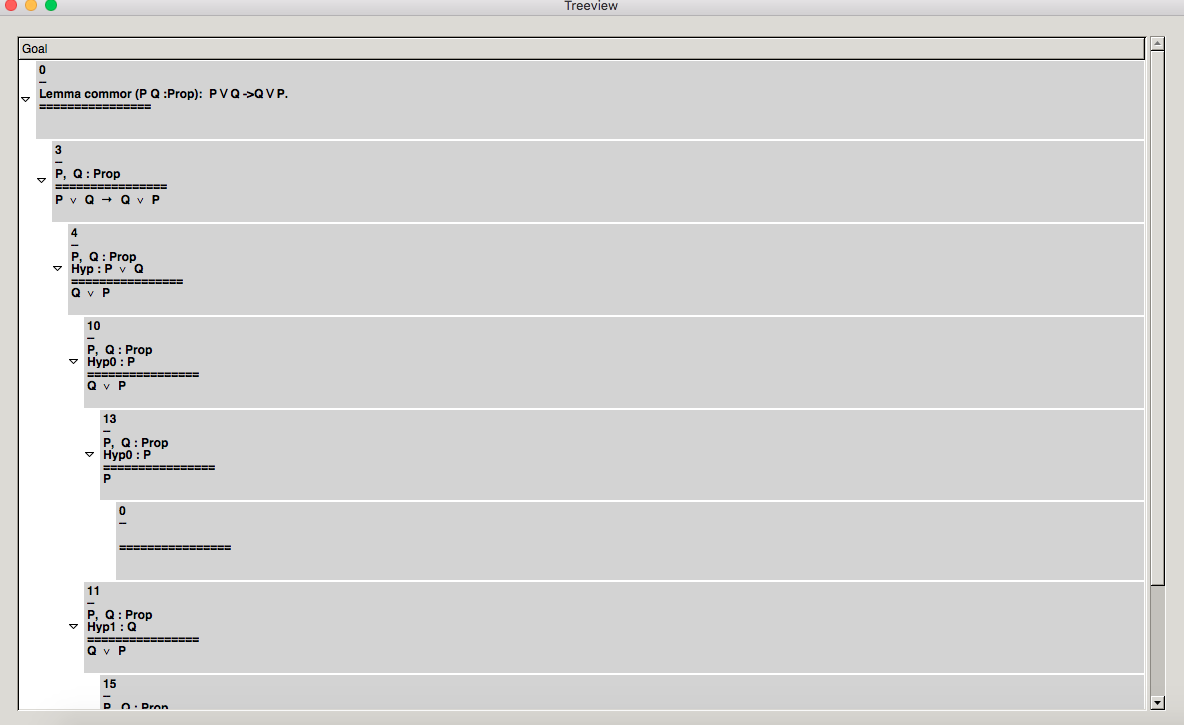
\includegraphics[scale=0.3]{Installation/treecommor.png}
\caption{the tree window}\label{treesearch}
\end{figure}

\subsection{An elementary number theory example}
We shall prove the transitivity of divisibility. That is we will prove that
$$\forall a,b, c \in \mathbb{N},  a |b \land b | c \Rightarrow a | c.$$

In the process we will introduce definitions and notations.

To start we note that we will be talking about objects of type \texttt{nat}. We weill introduce the following definition

\inp{Definition divides a b := exists x:nat, b = a*x.}

We hope that the format is quite clear, it resembles the one we used before but uses a few new notions, the operator \texttt{:=}
 which the defines the function \texttt{divides} and the quantifier \texttt{exists}. Note that we have not explicitly stated that a and b should be natural numbers, Coq will deduce that from the context. We could have been very precise as follows:
 \inp{ Definition divides (a b:nat) := exists x:nat, b = a*x.}

Note that the definition will not get any feedback from Coq. If we want to check that we have correctly defined our notion we can use
\inp{Check divides.}

to get

\mess{Query commands should not be inserted in
scripts\\

divides\\
     \texttt{: nat -> nat -> Prop}}
     
or
\inp{Print divides.}
to get a more detailed 
\mess{
Query commands should not be inserted in
scripts \\

divides = $\lambda a b : nat, \exists x : nat, b = a * x$\\
    \texttt{ : nat -> nat -> Prop}
\\
Argument scopes are [nat\_scope nat\_scope]
}
We will nod describe all this output here but we note the change from \texttt{exists} to $\exists$ and the occurrence of $\lambda$, a notation for functions.


Next we define a notation for divides

\inp{Notation " a | b " := (divides a b) (at level 10).}

Again no feedback from Coq. The definition should be self-evident except for the ``(at level 10)'' part. We will discuss this elsewhere.

We are now ready to state out theorem

We can state the theorem as (see the corresponding feedback)

\inp{Theorem refldiv (a b c:nat): \\ (a | b) $\land$ (b | c) -> (a |c).}

\coq{a,  b,  c : nat }{a  |  b  \land  b  |  c \rightarrow  a  |  c }

but we prefer the version

\inp{Theorem refldiv: forall a b c, (a | b) $\land$ (b | c) -> (a |c).
}
because it is  almost identical to the above mathematical statement and it will allow us to show some more tactics. The corresponding feedback is
\coq{ }{
\forall  a \  b\   c : nat,  a  |  b \  \land \ b  |  c\  \rightarrow\ a  |  c }

Note that Coq has correctly deduced that $a, b, c$ are natural numbers and replaced the quantifier \texttt{forall} with $\forall$. Note also that in this form there are no hypotheses.

We fill fix the three variables with the tactics:
\inp{Fix an arbitrary element a.\\
Fix an arbitrary element b.\\
Fix an arbitrary element c.}

to get 
\coq{a,  b,  c : nat \\
}{
a  |  b  \land  b  |  c \rightarrow  a  |  c }

As before, in order to prove an implication $A\rightarrow B$ we use the tactic

\inp{Assume A then prove B.}

More precisely, in this case we have
\inp{Assume (a | b $\land$ b | c ) then prove (a | c).}
to get

\coq {a,  b,  c : nat \\
Hyp : a  |  b  \land  b  |  c \\
}{
a  |  c }


Note that hypothesis Hyp is of type $A \land B$. We will split this in two hypotheses with:
\inp{Eliminate the conjuction in hypothesis Hyp.}
to get

\coq {a,  b,  c : nat \\
Hyp0 : a  |  b\\
Hyp1 :  b  |  c \\
}{
a  |  c }

We seem to have used all the tricks up our selves and so it is time to ``unfold'' the definitions:
\inp{Rewrite hypothesis Hyp0 using the definition of divides.}
\coq{a,  b,  c : nat \\
Hyp0 : \exists  x  :  nat,  b  =  a  *  x \\
Hyp1 :  b  |  c \\
}{
a  |  c }

then 
\inp{Rewrite hypothesis Hyp1 using the definition of divides.}
\coq{a,  b,  c : nat \\
Hyp0 : \exists  x  :  nat,  b  =  a  *  x \\
Hyp1 : \exists  x  :  nat,  c  =  b  *  x \\
}{
a  |  c }
and 

\inp{Rewrite goal using the definition of divides.}
\coq{a,  b,  c : nat \\
Hyp0 : \exists  x  :  nat,  b  =  a  *  x \\
Hyp1 : \exists  x  :  nat,  c  =  b  *  x \\
}{
\exists x : nat,  c  =  a  *  x  }


We now pick x as in the hypothesis Hyp1, that is:
\inp{Fix x the existentially quantified variable in Hyp1.}
to get 
\coq{a,  b,  c : nat \\
Hyp0 : \exists  x  :  nat,  b  =  a  *  x \\
x : nat \\
Hyp1 :   c  =  b  *  x \\
}{
\exists x0 : nat,  c  =  a  *  x0  }

Note the variable name was changed in the goal but not in Hyp0.

We now use the newly formed Hyp1 as follows:

\inp{Rewrite the goal using Hyp1.}

to get
\coq{a,  b,  c : nat \\
Hyp0 : \exists  x  :  nat,  b  =  a  *  x \\
x : nat \\
Hyp1 :   c  =  b  *  x \\
}{
\exists x0 : nat,  b  *  x  =  a  *  x0  }

Similarly we pick y as in Hyp0 and replace it in the goal

\inp{
Fix y the existentially quantified variable in Hyp0.\\
Rewrite the goal using Hyp0.
}

to get

\coq{a,  b,  c y : nat \\
Hyp0 :   b  =  a  *  y \\
x : nat \\
Hyp1 :   c  =  b  *  x \\
}{
\exists x0 : nat,  a  *  y  *  x  =  a  *  x0  }


It is now easy to guess that $x0 = y*x$ so we write

\inp{Prove the existential claim is true for (y*x).}

to obtain

\coq{a,  b,  c y : nat \\
Hyp0 :   b  =  a  *  y \\
x : nat \\
Hyp1 :   c  =  b  *  x \\
}{
 a  *  y  *  x  =  a  *  (y*x)  }

which can be proved by

\inp{True by arithmetic properties.}


the total proof is
\inp{
Definition divides (a b:nat) := exists x:nat, b = a*x. \\
Notation " a | b " := (divides a b) (at level 10).\\
Theorem refldiv:forall a b c, (a | b) $\land$ (b | c) -> (a |c).\\
Fix an arbitrary element a.\\
Fix an arbitrary element b.\\
Fix an arbitrary element c.
Assume (a | b $\land$ b | c ) then prove (a | c).\\
Eliminate the conjuction in hypothesis Hyp.\\
Rewrite hypothesis Hyp0 using the definition of divides.\\
Rewrite hypothesis Hyp1 using the definition of divides.\\
Rewrite goal using the definition of divides.\\
Fix x the existentially quantified variable in Hyp1.\\
Rewrite the goal using Hyp1.\\
Fix y the existentially quantified variable in Hyp0.\\
Rewrite the goal using Hyp0.\\
Prove the existential claim is true for (y*x).\\
True by arithmetic properties.
}

Note that one could use a slightly shorter version of this theorem:


\inp{Theorem refldiv (a b c:nat): (a | b) $\land$ (b | c) -> (a |c).\\
Rewrite goal using the definition of divides.\\
Assume $((\exists  x : nat,  b  =  a  *  x)  \land  (\exists  x  :  nat,  c  =  b  *  x)  )$ then prove $( \exists  x  :  nat,  c  =  a  *  x)$.\\
Eliminate the conjuction in hypothesis Hyp.\\
Fix x the existentially quantified variable in Hyp1.\\
Rewrite the goal using Hyp1.\\
Fix y the existentially quantified variable in Hyp0.\\
Rewrite the goal using Hyp0.\\
Prove the existential claim is true for (y*x).\\
True by arithmetic properties.}



Note also that if you save the latex form of the proof you will obtain the following:
\begin{tcolorbox}[colback=gray!10!white,colframe=white,breakable]
\begin{Definition}[divides] 
$divides\,(a\,b:nat)\,:=\,∃\,x:nat,\,b\,=\,a*x.
$
 \end{Definition}
\begin{Theorem}[refldiv] 
$\forall \,a\,b\,c,\,(a\,|\,b)\,\land (b\,|\,c)\,\Rightarrow \,(a\,|c).$
 \end{Theorem}
 Proof: In order to show $$\forall a b c : nat, a | b \land b | c \Rightarrow a | c $$ we pick an arbitrary $$a$$ and show $$\forall b c : nat, a | b \land b | c \Rightarrow a | c .$$
 In order to show $$\forall b c : nat, a | b \land b | c \Rightarrow a | c $$ we pick an arbitrary $$b$$ and show $$\forall c : nat, a | b \land b | c \Rightarrow a | c .$$
 In order to show $$\forall c : nat, a | b \land b | c \Rightarrow a | c $$ we pick an arbitrary $$c$$ and show $$a | b \land b | c \Rightarrow a | c .$$

 

 We will assume $$Hyp : a | b \land b | c $$ and show $$a | c .$$

 Since we know $$Hyp : a | b \land b | c $$ we also know $$Hyp0 : a | b 
Hyp1 : b | c .$$

 We use the definition of $$divides$$ in $$Hyp0$$ to obtain $$Hyp0 : \exists x : nat, b = a * x $$ 

 We use the definition of $$divides$$ in $$Hyp1$$ to obtain $$Hyp1 : \exists x : nat, c = b * x $$ 

 Rewriting the definition of $$divides$$ in our conclusion $$a | c $$, we now need to show $$\exists x : nat, c = a * x .$$

 We choose a variable $$x$$ in $$Hyp1$$ to obtain $$x : nat 
Hyp1 : c = b * x .$$

 We rewrite the goal using $$Hyp1$$ to obtain $$\exists x0 : nat, b * x = a * x0 .$$

 We choose a variable $$y$$ in $$Hyp0$$ to obtain $$a, b, c, y : nat 
Hyp0 : b = a * y .$$

 We rewrite the goal using $$Hyp0$$ to obtain $$\exists x0 : nat, a * y * x = a * x0 .$$

 We shall prove $$\exists x0 : nat, a * y * x = a * x0 $$ by showing $$a * y * x = a * (y * x) .$$

 This follows immediately from arithmetic.

 This is done Now $$a * y * x = a * (y * x) $$ means that $$\exists x0 : nat, a * y * x = a * x0 .$$ We have now proved $$\exists x0 : nat, a * y * x = a * x0 $$ and so $$\exists x0 : nat, b * x = a * x0 $$ follows. and so we have proved $$\exists x0 : nat, b * x = a * x0 .$$ We have now proved $$\exists x0 : nat, b * x = a * x0 $$ and so $$\exists x0 : nat, c = a * x0 $$ follows. and so we have proved $$\exists x : nat, c = a * x .$$ Therefore we have showed $$\exists x : nat, c = a * x $$ and so $$a | c .$$ therefore we have $$a | c .$$ therefore we have $$a | c .$$ We are now done with $$a | c .$$ We have now showed that if $$Hyp : a | b \land b | c $$ then $$a | c $$ a proof of $$a | b \land b | c \Rightarrow a | c .$$ Since $$c$$ was arbitrary this shows $$\forall c : nat, a | b \land b | c \Rightarrow a | c .$$ Since $$b$$ was arbitrary this shows $$\forall b c : nat, a | b \land b | c \Rightarrow a | c .$$ Since $$a$$ was arbitrary this shows $$\forall a b c : nat, a | b \land b | c \Rightarrow a | c .$$
 

\end{tcolorbox}


\bibliographystyle{plain-annote}
\bibliography{mybibliography}



\end{document}
\end

